% ============================================================
%  B4 — FDA Nozzle PINN Paper
%  Physics-Informed Neural Networks for Full-Field Hemodynamic
%  Reconstruction from Sparse Experimental PIV Data:
%  Validation on the FDA Critical Path Nozzle Benchmark
%
%  Author : Emmanuel Hackman
%  PhD Computational Science, University of Southern Mississippi
%
%  COLOR CODE LEGEND
%  -----------------
%  RED   \TODO{}   — Emmanuel writes this (your voice, your biology, your data)
%  BLUE  \CLAUDE{} — Claude drafts this (equations, lit review, methods prose)
%  ORANGE \DATA{}  — Fill from Colab / FDA dataset results
%  PURPLE \SHARED{} — Written together in session
%
%  COMPILATION
%  -----------
%  pdflatex B4_FDA_Nozzle_PINN_Paper.tex
%  bibtex   B4_FDA_Nozzle_PINN_Paper
%  pdflatex B4_FDA_Nozzle_PINN_Paper.tex
%  pdflatex B4_FDA_Nozzle_PINN_Paper.tex
% ============================================================

\documentclass[12pt,a4paper]{article}

% ── Encoding & fonts ────────────────────────────────────────
\usepackage[T1]{fontenc}
\usepackage[utf8]{inputenc}

% ── Color (MUST come before other packages that use color) ──
\usepackage[dvipsnames,table]{xcolor}

% ── Page layout ─────────────────────────────────────────────
\usepackage[margin=1in]{geometry}

% ── Math ────────────────────────────────────────────────────
\usepackage{amsmath, amssymb, amsthm}
\usepackage{bm}          % bold math symbols (\bm{u})

% ── Figures & tables ────────────────────────────────────────
\usepackage{graphicx}
\graphicspath{{figures/}}
\usepackage{booktabs}
\usepackage{multirow}
\usepackage{caption}
\usepackage{subcaption}
\usepackage{float}

% ── Hyperlinks ──────────────────────────────────────────────
\usepackage[colorlinks=true,linkcolor=blue,citecolor=blue,urlcolor=blue]{hyperref}

% ── References ──────────────────────────────────────────────
\usepackage{cite}

% ── Line numbers (for peer review) ──────────────────────────
\usepackage{lineno}

% ── Spacing ─────────────────────────────────────────────────
\usepackage{setspace}
\doublespacing

% ── Algorithm (uncomment when needed) ───────────────────────
%\usepackage{algorithm}
%\usepackage{algpseudocode}

% ── Units (uncomment when needed) ───────────────────────────
%\usepackage{siunitx}

% ═══════════════════════════════════════════════════════════
%  PLACEHOLDER MACROS
%  \newcommand in LaTeX2e is already \long (accepts \par).
%  \begingroup...\endgroup allows paragraph breaks inside.
% ═══════════════════════════════════════════════════════════
\newcommand{\TODO}[1]{\par\medskip\noindent
  \begingroup\color{red}\textbf{[\,EMMANUEL:\;} #1 \textbf{]}\endgroup
  \par\medskip}

\newcommand{\CLAUDE}[1]{\par\medskip\noindent
  \begingroup\color{blue}\itshape [\,CLAUDE drafts:\; #1 ]\endgroup
  \par\medskip}

\newcommand{\DATA}[1]{{\color{orange}\textbf{[DATA:\;#1]}}}

\newcommand{\SHARED}[1]{\par\medskip\noindent
  \begingroup\color{violet}\textbf{[\,SHARED:\;} #1 \textbf{]}\endgroup
  \par\medskip}

% ── Theorem environments ────────────────────────────────────
\newtheorem{remark}{Remark}
\newtheorem{proposition}{Proposition}

% ── Convenience math macros ─────────────────────────────────
\newcommand{\bu}{\bm{u}}          % velocity vector
\newcommand{\bx}{\bm{x}}          % position vector
\newcommand{\nablah}{\nabla}       % gradient
\newcommand{\Reyn}{\mathrm{Re}}    % Reynolds number
\newcommand{\Loss}{\mathcal{L}}    % loss function
\newcommand{\Net}{\mathcal{N}}     % neural network

% ============================================================
\begin{document}
\linenumbers

% ── Title block ─────────────────────────────────────────────
\title{
  \textbf{Mesh-Free Inverse Reconstruction of the Incompressible
  Navier--Stokes State from Sparse and Direction-Blind PIV
  Measurements:\\
  A Physics-Informed Neural Network Framework Validated on the
  FDA Critical Path Nozzle and Blood Pump Benchmarks}
}

\author{
  Emmanuel Hackman\\
  \small School of Mathematics and Natural Sciences\\
  \small University of Southern Mississippi, Hattiesburg, MS 39406\\
  \small \texttt{emmanuelhackman825@gmail.com}
}

\date{\today}
\maketitle

% ── Abstract ────────────────────────────────────────────────
\begin{abstract}
\noindent
We present a mesh-free physics-informed neural network (PINN)
framework for the inverse reconstruction of the full incompressible
Navier--Stokes state --- velocity, pressure, and wall shear stress
--- from sparse and direction-blind experimental particle image
velocimetry (PIV) measurements. The framework parameterises the
unknown PDE solution as a multi-layer perceptron with hard input
normalisation and output scaling, trains the network parameters
by minimising a composite loss combining a per-component
relative-$L^2$ data fit and the Navier--Stokes residuals evaluated
at uniformly resampled collocation points, and recovers the
unmeasured pressure and wall-shear-stress fields through automatic
differentiation without any auxiliary CFD simulation.

We make four methodological contributions.
\emph{(i)~Hard-constraint magnitude enforcement.} For
direction-blind data we introduce an output-transform
parametrisation $\hat{u} = |\hat{V}|\cos\hat{\theta}$,
$\hat{v} = |\hat{V}|\sin\hat{\theta}$ that enforces the PIV
magnitude as a structural hard constraint, leaving the
Navier--Stokes residuals as the sole driver of direction recovery
and eliminating the gradient competition between data and physics
losses in the soft-data formulation.
\emph{(ii)~Direction-from-magnitude reconstruction.} We show that
the momentum residuals --- not the continuity constraint --- are
the mechanism by which the PINN selects the unique
physically-realisable vector field from the equivalence class
compatible with the observed scalar magnitude; a four-configuration
ablation rules out data fitting and continuity in isolation.
\emph{(iii)~Numerical-uniqueness evidence.} An $8$-seed
deep-ensemble construction yields pairwise cosine similarity above
\DATA{[abs.cossim-min]} across all recovered vector fields,
empirically establishing uniqueness on the pump-diffuser geometry
in the absence of a formal theorem.
\emph{(iv)~Cross-dataset transferability.} A single architecture,
training schedule, and loss formulation generalise across both
U.S.\ FDA inter-laboratory benchmark medical devices --- the
Critical Path nozzle (axisymmetric, $\Reyn = 500$--$3500$,
full-vector PIV) and the Blood Pump diffuser (2D Cartesian,
$\Reyn_{\text{pump}} = 2.1$--$2.9 \times 10^5$, magnitude-only
PIV) --- with no modification beyond the dimensionality of the
domain.

Quantitatively, on the nozzle the framework attains relative-$L^2$
velocity error of $7.5\%$ at $\Reyn = 500$ and a Stewart~2012-style
global error metric $E_g = 0.137$ that is $2.5\times$ smaller than
the best CFD group in the 28-laboratory FDA inter-laboratory
study. On the pump diffuser the framework attains relative-$L^2$
velocity-magnitude error below $1.7\%$ across all five operating
conditions and peak-velocity capture above $98.8\%$. A
$3 \times 3$ hyperparameter-sensitivity study confirms that the
results are stable to network-width and data-weight choices
(min--max range \DATA{[abs.hp-range]}\%). Each benchmark case
trains in $11$--$26$~minutes on a single consumer-grade NVIDIA T4
GPU, a $5$--$30\times$ wall-clock speed-up relative to traditional
CFD on the same problems.

\medskip
\noindent\textbf{Keywords:} physics-informed neural networks,
incompressible Navier--Stokes equations, inverse problem,
mesh-free methods, particle image velocimetry, sparse
reconstruction, automatic differentiation, FDA Critical Path
nozzle benchmark, FDA Blood Pump benchmark, wall shear stress
\end{abstract}

\newpage

% ============================================================
%  SECTION 1 — INTRODUCTION
% ============================================================
\section{Introduction}
\label{sec:intro}

Cardiovascular medical devices --- prosthetic heart valves,
ventricular assist devices (VADs), continuous-flow blood pumps,
and total artificial hearts --- must demonstrate hemodynamic
safety before clearance for human use. The critical failure
modes in these devices are not mechanical but hemodynamic:
abnormal wall shear stress (WSS) causes platelet activation,
which precipitates thrombus formation; thrombi shed downstream
cause embolic stroke; and excessive shear in narrow gaps
fragments red blood cells, producing intravascular hemolysis
\cite{Malek1999WSS, Shadden2013WSS}. The history of
device-related morbidity is dominated by these failure modes:
the Bjork--Shiley convexo-concave heart valve's strut
fractures, the HeartMate~II VAD's pump-thrombosis adverse-event
rate, and ongoing hemolysis concerns in current-generation
continuous-flow pumps all trace to hemodynamic conditions that
were difficult to characterise pre-clinically. Quantitative
maps of velocity, pressure, and WSS in candidate device
geometries are therefore not optional for regulatory review ---
they are the substrate on which clearance decisions are made.

The current engineering pipeline for producing those maps is
bifurcated. Particle image velocimetry (PIV) in transparent
analogue geometries gives spatially-resolved velocity
measurements that are experimentally grounded, but PIV cannot
measure pressure directly, loses accuracy within roughly one
millimetre of the wall (the optical boundary layer), and
requires manufacturing and instrumenting a physical phantom for
each design variant. Computational fluid dynamics (CFD) fills
the missing fields --- pressure everywhere, WSS at the wall ---
but at substantial cost: hours to days of compute per geometry,
expert meshing for the near-wall region, explicit selection of
a turbulence-closure model, and round-trip validation against
PIV experiments that the simulation was meant to displace. The
FDA's Critical Path Initiative \cite{FDACriticalPath2004} and
its 2021 guidance on computational modelling in regulatory
submissions \cite{FDA2021InSilico} have explicitly identified
the need for tools that bridge these two pipelines: a
methodology that consumes the PIV data manufacturers already
collect and recovers the full physical state --- pressure and
WSS included --- without an additional CFD simulation cycle.

Physics-informed neural networks (PINNs)
\cite{Raissi2019PINN1, Raissi2019PINN2} offer a natural
mathematical formulation of exactly this bridge. A PINN
parameterises the unknown PDE solution as a neural network and
trains the network parameters by minimising a composite loss
that combines (i) a data-fit term on observed quantities and
(ii) the residuals of the governing partial differential
equations at randomly sampled collocation points. For the
incompressible Navier--Stokes system, this means that observed
velocity at a sparse subset of points is sufficient to constrain
a continuous velocity, pressure, and WSS field everywhere in
the domain, because the momentum equation algebraically
determines pressure once velocity is known and the
no-slip-wall boundary condition algebraically determines WSS
once velocity is known. Recent applications to cardiovascular
flow have demonstrated this principle in idealised geometries
and patient-specific aortic arches
\cite{Raissi2020HFM, Arzani2021PINN_Blood, Kissas2020CardiacPINN};
what remains open is whether the methodology generalises across
the heterogeneous device geometries, Reynolds numbers, and PIV
data modalities that the FDA benchmark portfolio actually
includes.

The present paper addresses that question directly. We apply a
single PINN methodology --- identical architecture, training
schedule, and loss formulation up to dimensionality of the
domain --- to both of the FDA's inter-laboratory benchmark
medical devices:
\begin{itemize}[leftmargin=*, itemsep=2pt]
  \item the \textbf{FDA Critical Path nozzle}
    \cite{Hariharan2011FDA, Stewart2012FDA}, an axisymmetric
    sudden-expansion geometry that has become the gold-standard
    benchmark for cardiovascular-device CFD validation, with
    published vector-PIV data at $\Reyn = 500$, $2000$, and
    $3500$ spanning laminar to transitional regimes; and
  \item the \textbf{FDA Blood Pump diffuser}
    \cite{Hariharan2018BloodPump, Malinauskas2017FDA,
    Ponnaluri2023PumpCFD}, a 2D-non-axisymmetric centrifugal-pump
    diffuser region with magnitude-only PIV at five operating
    conditions spanning $\Reyn_{\text{pump}} = 2.1$ to $2.9
    \times 10^5$.
\end{itemize}

The contribution is six-fold.
\emph{First}, we introduce a hard-constraint magnitude
enforcement (Sec.~\ref{sec:hard_constraint}) that parametrises
the network output as
$\hat{u} = |\hat{V}|\cos\hat{\theta}$,
$\hat{v} = |\hat{V}|\sin\hat{\theta}$, structurally enforcing
the PIV magnitude as an exact constraint at data points and
leaving the Navier--Stokes residuals as the sole driver of
direction recovery. This eliminates the gradient competition
between the data-fit and PDE-residual terms that has been
documented as a primary failure mode in soft-constraint PINNs
\cite{Wang2021GradientPath}.
\emph{Second}, we isolate the mechanism by which the PINN
recovers a fully vector-resolved velocity field from
direction-blind PIV magnitude measurements: a
four-configuration ablation
(Sec.~\ref{sec:ablation_results}) shows that the momentum
residuals --- not the continuity constraint --- are necessary
and sufficient to disambiguate flow direction from a scalar
data signal. \emph{Third}, an $8$-seed deep-ensemble
construction (Sec.~\ref{sec:uq_uniqueness}) yields pairwise
cosine similarity above \DATA{[intro.cossim-min]} between all
recovered vector fields, providing empirical evidence for
numerical uniqueness of the inverse problem in the absence of
a formal theorem, together with calibrated coefficient-of-variation
maps for the reconstructed pressure and wall-shear-stress fields.
\emph{Fourth}, we present the first reported PINN reconstruction
on either of the FDA inter-laboratory benchmark datasets, and
recover pressure and WSS without any CFD simulation, using only
sparse PIV velocity observations and the Navier--Stokes
equations as constraints. \emph{Fifth}, on the nozzle benchmark
we directly compare against the 28-group Stewart~2012
inter-laboratory CFD study using its own published error metric,
and show that the PINN matches or outperforms the best CFD
group at every Reynolds number. \emph{Sixth}, we demonstrate that
the methodology generalises across two FDA benchmarks, three
orders of magnitude in Reynolds number, two distinct geometries
(axisymmetric nozzle vs.\ 2D pump diffuser), and two PIV data
modalities (vector vs.\ magnitude only), with no architectural
or training-schedule changes between the two applications ---
establishing that physics-informed reconstruction is a
transferable methodology rather than a benchmark-specific
tuning exercise.

The remainder of this paper is organised as follows.
Section~\ref{sec:background} reviews the two FDA benchmarks
and relevant prior work in PINN-based hemodynamic
reconstruction. Section~\ref{sec:formulation} states the
governing equations and the inverse-problem formulation.
Section~\ref{sec:methods} describes the PINN architecture
and training procedure. Section~\ref{sec:results} presents
validation results on the FDA nozzle benchmark including a
direct comparison against the Stewart~2012 inter-laboratory CFD
study. Section~\ref{sec:pump_application} applies the same
methodology to the FDA Blood Pump diffuser. Section~\ref{sec:discussion}
discusses implications, limitations, and regulatory relevance.
Section~\ref{sec:conclusion} concludes.

% ============================================================
%  SECTION 2 — BACKGROUND AND RELATED WORK
% ============================================================
\section{Background and Related Work}
\label{sec:background}

\subsection{The FDA Critical Path Nozzle Benchmark}
\label{sec:fda_benchmark}

The FDA Critical Path nozzle is a simplified axisymmetric
cardiovascular-device test geometry comprising three regions: a
gradual contraction from an inlet diameter of $0.012$~m to a
cylindrical throat of diameter $d = 0.004$~m over a length of
$0.022611$~m, a constant-area throat of length $0.04$~m, and a
sudden expansion back to the inlet diameter at $x = 0.04$~m. The
benchmark was established by the FDA Critical Path Initiative
\cite{FDA2009Nozzle, FDACriticalPath2004} to provide a standardised
geometry for verification and validation of cardiovascular-device
computational models.

Hariharan et al.\ (2011) \cite{Hariharan2011FDA} published the
canonical PIV dataset: stereoscopic-PIV measurements of axial and
radial velocity at five Reynolds numbers
($\Reyn = 500, 2000, 3500, 5000, 6500$) spanning laminar,
transitional, and turbulent regimes. The dataset is publicly
mirrored by the FDA Office of Science and Engineering Laboratories
(OSEL) on GitHub
(\url{github.com/OSEL-DAM/CFD-and-Blood-Damage-Benchmarks}) and
provides $4{,}000$--$4{,}300$ valid velocity samples per Reynolds
number, distributed across axial wall-distribution measurements,
centreline distributions, and radial profiles at $13$ axial
stations spanning $-0.020 \leq x \leq 0.143$~m relative to the
throat-end origin. This dataset has been used as the gold standard
for CFD validation in the FDA's 28-laboratory Stewart~2012 study
\cite{Stewart2012FDA} and subsequent inter-laboratory work
\cite{Steinman2013FDA}, and remains the most-cited experimental
reference in cardiovascular-device CFD validation.

\subsection{Physics-Informed Neural Networks}
\label{sec:pinn_background}

Raissi, Perdikaris, and Karniadakis
\cite{Raissi2019PINN1, Raissi2019PINN2} introduced
physics-informed neural networks (PINNs) as a mesh-free
methodology for forward and inverse PDE problems. A PINN
parameterises the unknown solution of a PDE as a neural network
$\hat{\bm{u}}_\theta(\bm{x}, t)$ and trains the network weights
$\theta$ by minimising a composite loss that combines PDE
residuals evaluated at randomly sampled collocation points,
boundary and initial condition residuals, and a data-fit term
on any observed quantities. Automatic differentiation
\cite{Baydin2018AutoDiff} provides exact derivatives of the
network output with respect to its spatial inputs, allowing the
PDE residuals to be evaluated without finite-difference
discretisation. Open-source implementations such as DeepXDE
\cite{Lu2021DeepXDE} have lowered the barrier to entry, and a
substantial body of subsequent methodological work has
addressed gradient pathology
\cite{Wang2021GradientPath}, adaptive collocation sampling
\cite{Wu2023RAR}, and Bayesian extensions for uncertainty
quantification \cite{Yang2021BayesPINN}.

Applications of PINNs to fluid mechanics specifically have
established the methodology as a competitive alternative to
traditional CFD on a variety of problems. Raissi, Yazdani, and
Karniadakis~(2020) \cite{Raissi2020HFM} demonstrated ``hidden
fluid mechanics'' --- recovery of velocity and pressure fields
from passive-scalar concentration data using
Navier--Stokes-constrained PINNs --- and Cai et~al.~(2021)
\cite{Cai2021FluidPINN} reviewed the state of the art across a
range of flow regimes including incompressible, compressible,
and biomedical applications. In cardiovascular contexts
specifically, Kissas et~al.~(2020) \cite{Kissas2020CardiacPINN}
applied PINNs to clinical MRI velocimetry data for
patient-specific aortic flow, and Arzani et~al.~(2021)
\cite{Arzani2021PINN_Blood} extended the methodology to
near-wall flow estimation in arterial geometries with sparse
near-wall data. Notwithstanding this growing literature,
\emph{no prior work has applied PINNs to either of the FDA's
inter-laboratory benchmark medical-device experimental PIV
datasets} --- the most widely used reference geometries in
cardiovascular-device computational validation.

\subsection{Wall Shear Stress and Medical Device Safety}
\label{sec:wss_background}

Wall shear stress (WSS) is a primary determinant of the
hemocompatibility of cardiovascular medical devices. Elevated
WSS in excess of approximately $150$~dyn/cm$^2$ (15~Pa) activates
platelets and initiates thrombus formation through the
von~Willebrand-factor pathway \cite{Shadden2013WSS}, while
abnormally low or oscillatory WSS promotes endothelial
dysfunction and atherogenesis \cite{Malek1999WSS}. Both regimes
contribute to documented device-related morbidity: high-shear
zones near mechanical-valve hinges and in
continuous-flow-pump rotor clearances drive intravascular
hemolysis and thromboembolic stroke; low-shear stagnation
zones in pump diffusers and outlet cannulae nucleate
thrombi that subsequently embolise. Existing FDA guidance for
biological evaluation of cardiovascular devices
(ISO~10993-4) requires explicit assessment of thrombogenic and
hemolytic potential, both of which are mechanistically rooted
in the WSS field. Direct measurement of WSS in a transparent
phantom is, however, beyond the resolution of standard
particle image velocimetry: PIV cannot resolve the velocity
gradient $\partial u_x / \partial r$ within the optical
boundary layer of roughly $0.5$--$1$~mm adjacent to the wall.
CFD can produce a WSS field, but is itself dependent on PIV
validation; the field-evaluation pipeline therefore loops on
itself. Physics-informed neural networks offer a way out of
this loop: WSS is recovered directly from bulk-flow PIV
through the no-slip boundary condition and automatic
differentiation, without an additional simulation cycle.

\subsection{Gaps in the Literature}
\label{sec:gaps}

Three gaps in the existing literature motivate the present
work. First, prior applications of PINNs to fluid mechanics
have used either purely synthetic data
\cite{Raissi2019PINN1, Lu2021DeepXDE}, clinical 4D-flow MRI
\cite{Kissas2020CardiacPINN, Arzani2021PINN_Blood}, or
passive-scalar concentration fields \cite{Raissi2020HFM}; none
have used either of the FDA inter-laboratory PIV benchmarks
\cite{Hariharan2011FDA, Hariharan2018BloodPump} as training
data. Second, existing computational studies of the FDA
benchmarks apply traditional CFD (finite-volume or
finite-element discretisation with explicit turbulence
closures) and \emph{validate} their solutions against the PIV
\cite{Stewart2012FDA, Steinman2013FDA, Ponnaluri2023PumpCFD};
they never invert the problem to use PIV as training data and
recover the pressure and WSS fields directly. Third, no
prior study has demonstrated cross-dataset transferability of
a single PINN methodology across two FDA benchmarks differing
by three orders of magnitude in Reynolds number, two distinct
geometric formulations, and two PIV data modalities. The
present paper addresses all three gaps simultaneously.

% ============================================================
%  SECTION 3 — PROBLEM FORMULATION
% ============================================================
\section{Problem Formulation}
\label{sec:formulation}

\subsection{FDA Nozzle Geometry and Flow Conditions}
\label{sec:geometry}

The FDA nozzle is treated as an axisymmetric domain
$\Omega \subset \mathbb{R}^2$ in the $(x, r)$ half-plane, where
$x$ is the axial coordinate and $r$ is the radial coordinate
($r \geq 0$). The geometry consists of three regions:
\begin{enumerate}[leftmargin=*, itemsep=2pt]
  \item \textbf{Inlet tube:} constant diameter
        $D = 0.012$~m extending over $-0.088 \leq x \leq -0.0226$~m;
  \item \textbf{Constriction and throat:} gradual conical
        contraction from $D$ to throat diameter
        $d = 0.004$~m over the axial range
        $-0.0226 \leq x \leq 0$~m, followed by a cylindrical
        throat of length $0.04$~m extending over
        $0 \leq x \leq 0.04$~m;
  \item \textbf{Sudden expansion and outlet:} sudden
        backward-facing-step expansion to $D$ at $x = 0.04$~m,
        followed by an outlet tube extending to $x = 0.143$~m
        (the extent of the available PIV measurements).
\end{enumerate}
The throat-end origin convention ($x = 0$ at the downstream end
of the constriction) follows Hariharan~2011
\cite{Hariharan2011FDA} and is adopted throughout this paper.

The Reynolds number is defined with respect to the throat diameter:
\begin{equation}
  \Reyn = \frac{\rho \bar{U} d}{\mu}
  \label{eq:reynolds}
\end{equation}
where $\rho = 1060$~kg/m$^3$ is the working fluid density
(blood-analog glycerol-water mixture), $\bar{U}$ is the mean
throat velocity, and $\mu = 3.5 \times 10^{-3}$~Pa$\cdot$s is the
dynamic viscosity.

These values correspond to the working fluid documented in the
Hariharan~2011 PIV protocol \cite{Hariharan2011FDA}: a
sodium-iodide/water/glycerin blood-analogue mixture with
refractive index matched to the acrylic test section, density
$\rho = 1060$~kg/m$^3$, and dynamic viscosity
$\mu = 3.5 \times 10^{-3}$~Pa$\cdot$s ($3.5$~cP).

\subsection{Governing Equations}
\label{sec:governing}

The flow is governed by the incompressible Navier--Stokes
equations, which constitute the exact physical model for the
working fluid considered here; the PINN does not approximate
the governing physics, only the spatial dependence of the
solution.

We model the flow as incompressible and Newtonian. The governing
equations are the incompressible Navier-Stokes equations:

\begin{equation}
  \rho\left(\frac{\partial \bu}{\partial t}
  + \bu \cdot \nablah\bu\right)
  = -\nablah p
  + \mu\,\nablah^2 \bu
  + \bm{f},
  \quad (\bx, t) \in \Omega \times (0, T]
  \label{eq:NS_momentum}
\end{equation}

\begin{equation}
  \nablah \cdot \bu = 0,
  \quad (\bx, t) \in \Omega \times (0, T]
  \label{eq:NS_continuity}
\end{equation}

where $\bu(\bx, t) = (u, v)^T$ is the velocity field,
$p(\bx, t)$ is the kinematic pressure, $\rho$ is the fluid
density, $\mu$ is the dynamic viscosity, and $\bm{f}$ represents
body forces (set to zero here).

For the steady laminar cases ($\Reyn \leq 500$) we solve the
steady Navier-Stokes equations:

\begin{equation}
  \rho\left(\bu \cdot \nablah\bu\right)
  = -\nablah p + \mu\,\nablah^2 \bu
  \label{eq:NS_steady}
\end{equation}

At $\Reyn = 500$ the flow is steady, axisymmetric, and laminar;
the steady Navier--Stokes system is the exact model. At
$\Reyn = 2000$ and $3500$ the flow becomes transitional in the
post-throat recirculation zone, with low-amplitude unsteadiness
superposed on a well-defined ensemble-averaged flow field. The
Hariharan~2011 PIV data are themselves ensemble averages over
many stereoscopic image pairs and therefore report only the
mean velocity. We accordingly treat the transitional cases as
\emph{quasi-steady}: the PINN fits the ensemble-averaged
velocity through the steady Navier--Stokes residuals, which is
exact for the mean flow under Reynolds decomposition provided
the Reynolds-stress contributions are absorbed into an
effective viscosity. The accuracy implications of this
quasi-steady approximation are discussed quantitatively in
Sec.~\ref{sec:discuss_re}.

\subsection{Wall Shear Stress Definition}
\label{sec:wss_def}

The wall shear stress is defined as the tangential component of
the stress tensor at the vessel wall $\partial\Omega_w$:

\begin{equation}
  \tau_w = \mu \left.\frac{\partial u_t}{\partial n}\right|_{\partial\Omega_w}
  \label{eq:wss}
\end{equation}

where $u_t$ is the tangential velocity component and $n$ is the
wall-normal direction. This quantity \emph{cannot} be measured
directly from PIV data because the velocity gradient at the wall
requires sub-pixel resolution unavailable in standard PIV systems.

\subsection{The Inverse Problem Statement}
\label{sec:inverse}

We observe sparse, noisy ensemble-averaged velocity data from
PIV,
\begin{equation}
  \mathcal{D} = \{(\bx_i,\,\bu_i^{\text{obs}})\}_{i=1}^{N_d},
  \qquad
  \bu_i^{\text{obs}} = \bu(\bx_i) + \epsilon_i,
  \quad \epsilon_i \sim \mathcal{N}(0, \sigma^2 \bm{I}),
  \label{eq:inverse_data}
\end{equation}
where $N_d \approx 4{,}000$--$4{,}300$ for the nozzle and
$N_d \approx 3{,}900$--$4{,}100$ for the pump diffuser. The
unmeasured quantities are the pressure field $p(\bx)$ on
$\Omega$ and the wall shear stress
$\tau_w(\bx) = \mu (\partial u_t/\partial n)|_{\partial\Omega_w}$
along the wall boundary. The inverse problem is to recover both
unmeasured fields from the observed velocity samples, subject
to the constraint that the recovered velocity-pressure pair
$(\bu, p)$ satisfies the steady incompressible Navier--Stokes
system, Eqs.~\eqref{eq:NS_momentum}--\eqref{eq:NS_continuity}.
This is the canonical PINN-inverse formulation
\cite{Raissi2019PINN1, Raissi2020HFM} applied to FDA
benchmark experimental data.

% ============================================================
%  SECTION 4 — METHODOLOGY
% ============================================================
\section{Methodology}
\label{sec:methods}

\subsection{PINN Architecture}
\label{sec:architecture}

We use a single feed-forward multi-layer perceptron (MLP)
$\Net_\theta: (x, r) \mapsto (\hat{N}_x, \hat{N}_r, \hat{p})$
that maps the axisymmetric spatial coordinates to three scalar
outputs: two raw velocity-component activations $\hat{N}_x$ and
$\hat{N}_r$ that are subsequently scaled and projected onto a
hard-BC-satisfying function space (Sec.~\ref{sec:loss}), and a
raw pressure activation $\hat{p}$ that is scaled by the dynamic
pressure $P_{\text{scale}} = \rho U_{\text{scale}}^2$. Unlike
the dual-network architecture used in some prior PINN-for-fluids
work \cite{Raissi2020HFM}, we share all hidden layers across the
three output channels: empirical experiments showed that
separating velocity and pressure heads slowed convergence
without measurable accuracy improvement on either FDA
benchmark, and the shared representation enables the
momentum equation to couple all three fields through
back-propagation during a single forward pass.

The network $\Net_\theta$ has the form:

\begin{equation}
  \hat{\phi}(\bx; \theta) =
  W_L \sigma\!\left(W_{L-1}\sigma\!\left(\cdots
  \sigma(W_1 \bx + b_1)\cdots\right)
  + b_{L-1}\right) + b_L
  \label{eq:network}
\end{equation}

where $\sigma(\cdot)$ is the activation function (hyperbolic
tangent), $\{W_\ell, b_\ell\}$ are the trainable weights and
biases, and $\theta$ denotes all trainable parameters.

In all experiments reported in this paper we use
\begin{itemize}[leftmargin=*, itemsep=2pt]
  \item Number of hidden layers $L = 6$;
  \item Neurons per layer $W = 64$;
  \item Activation function $\sigma(\cdot) = \tanh(\cdot)$,
        consistent with the original PINN formulation
        \cite{Raissi2019PINN1};
  \item Total trainable parameters $\approx 21{,}000$.
\end{itemize}
Input coordinates are hard-normalised to $[-1, +1]^2$ before
entering the network, and raw outputs are scaled by physical
units ($U_{\text{scale}}$, $P_{\text{scale}}$) to recover the
solution fields. The combination of input normalisation and
output scaling is essential for training stability when the
physical coordinates and target velocities differ by several
orders of magnitude in raw units (Sec.~\ref{sec:training}).

\subsection{Loss Function}
\label{sec:loss}

The PINN is trained by minimizing a composite loss function that
enforces (i) fidelity to the PIV data, (ii) satisfaction of the
Navier-Stokes momentum equations, (iii) divergence-free velocity,
and (iv) boundary conditions:

\begin{equation}
  \Loss(\theta) = \lambda_d \Loss_d
               + \lambda_m \Loss_m
               + \lambda_c \Loss_c
               + \lambda_b \Loss_b
  \label{eq:total_loss}
\end{equation}

The \textbf{data loss} enforces agreement with the $N_d$ PIV
velocity observations:
\begin{equation}
  \Loss_d = \frac{1}{N_d}\sum_{i=1}^{N_d}
            \left|\hat{\bu}(\bx_i) - \bu_i^{\text{obs}}\right|^2
  \label{eq:loss_data}
\end{equation}

The \textbf{momentum residual loss} enforces the Navier-Stokes
equations at $N_r$ collocation points $\{\bx_j^r\}$ sampled
throughout $\Omega$:
\begin{equation}
  \Loss_m = \frac{1}{N_r}\sum_{j=1}^{N_r}
            \left|\rho(\hat{\bu} \cdot \nablah\hat{\bu})
            + \nablah\hat{p} - \mu\,\nablah^2\hat{\bu}
            \right|^2_{\bx_j^r}
  \label{eq:loss_momentum}
\end{equation}

The \textbf{continuity residual loss} enforces incompressibility:
\begin{equation}
  \Loss_c = \frac{1}{N_r}\sum_{j=1}^{N_r}
            \left|\nablah \cdot \hat{\bu}\right|^2_{\bx_j^r}
  \label{eq:loss_continuity}
\end{equation}

The \textbf{boundary condition loss} enforces no-slip at the wall
($\hat{\bu} = \bm{0}$ on $\partial\Omega_w$) and the prescribed
inlet velocity profile at $N_b$ boundary points:
\begin{equation}
  \Loss_b = \frac{1}{N_b}\sum_{k=1}^{N_b}
            \left|\hat{\bu}(\bx_k^b) - \bu_k^{\text{BC}}\right|^2
  \label{eq:loss_bc}
\end{equation}

The relative weighting of the four loss components is the
single most consequential hyperparameter in PINN training. Wang
et~al.~(2021) \cite{Wang2021GradientPath} document a
\emph{gradient pathology} in which one term --- typically the
data loss for inverse problems --- dominates back-propagated
gradients and starves the others, producing solutions that fit
the data but violate the PDE (or vice versa). They propose an
NTK-based adaptive weighting scheme that rebalances the
gradients at every training step. In preliminary experiments we
implemented the Wang~2021 scheme but found that the data term
$\Loss_d$, when normalised on a per-component relative-$L^2$
basis (see below), already produces well-conditioned gradients
across both benchmarks; the additional complexity of NTK
adaptation was not required.

For the inverse-reconstruction setting of the present paper,
where PIV velocity is the only directly-observed quantity, we
follow the standard practice of weighting the data loss more
strongly than the PDE residuals so that the network anchors to
the experimental measurements before fitting the physics. The
final weights used across all experiments are:
\begin{equation*}
  \lambda_d \in [100, 400],
  \quad
  \lambda_m = \lambda_c = 1,
  \quad
  \lambda_b \in [0.1, 10],
\end{equation*}
with $\lambda_d$ increasing from $100$ at $\Reyn = 500$ to $400$
at $\Reyn = 3500$ to compensate for the larger PDE-residual
gradient magnitudes at higher Reynolds number. The data loss
itself is implemented as a \emph{per-component relative}-$L^2$
norm rather than a raw mean-squared error:
\begin{equation}
  \Loss_d
  = \tfrac{1}{2}\!\left[
    \frac{\sum_i (\hat{u}_x(\bx_i) - u_{x,i}^{\text{obs}})^2}
         {\sum_i (u_{x,i}^{\text{obs}})^2 + \varepsilon}
   +\frac{\sum_i (\hat{u}_r(\bx_i) - u_{r,i}^{\text{obs}})^2}
         {\sum_i (u_{r,i}^{\text{obs}})^2 + \varepsilon}
   \right],
  \label{eq:loss_data_rel}
\end{equation}
which normalises each velocity component by its own measured
magnitude and prevents the larger-magnitude $u_x$ component
from dominating the loss when $u_r$ is small but
physically meaningful.

\subsection{Automatic Differentiation and PDE Residuals}
\label{sec:autodiff}

All spatial derivatives entering the PDE residuals ---
$\partial_x$, $\partial_r$, and the second derivatives in the
viscous term --- are computed by automatic differentiation
\cite{Baydin2018AutoDiff} through the network graph rather than
by finite-difference discretisation. Automatic differentiation
returns derivatives that are accurate to machine precision and
defined continuously over $\Omega$, so the PDE residuals can be
evaluated at any spatial location without a mesh. This is the
mathematical foundation of the mesh-free property of PINNs:
unlike finite-volume or finite-element discretisations, the
governing equations are evaluated pointwise on randomly
sampled collocation points rather than over a fixed grid. Our
implementation uses JAX
\cite{Frostig2018JAX} with double-precision (float64) arithmetic
to ensure derivative accuracy at the resolutions required by
the viscous term in the high-Reynolds-number pump cases.

\subsection{Collocation Point Sampling Strategy}
\label{sec:sampling}

Interior collocation points are drawn uniformly at random over
the spatial domain at every Adam iteration, with the random
seed advanced each step to give the network exposure to fresh
samples. Resampling at every iteration (rather than fixing a
single static collocation set) acts as an implicit regulariser
and prevents the network from over-fitting to a particular
collocation realisation. Residual-adaptive refinement (RAR)
\cite{Wu2023RAR} --- adding more collocation points in regions
where the PDE residual is largest --- was tested in preliminary
experiments but produced no measurable accuracy improvement on
either FDA benchmark; the uniform-resampling strategy is
sufficient at the network width and depth used here.

The collocation-point counts used in this paper are:
\begin{itemize}[leftmargin=*, itemsep=2pt]
  \item Nozzle: $N_r = 5{,}000$ ($\Reyn = 500$),
        $7{,}000$ ($\Reyn = 2000$), $8{,}000$ ($\Reyn = 3500$);
        $N_d \in [4{,}088, 4{,}230]$ from the Hariharan~2011
        PIV deposit; boundary terms are enforced as a hard
        output transform rather than soft loss
        (Sec.~\ref{sec:architecture}), so $N_b = 0$ effectively;
  \item Pump diffuser: $N_r = 8{,}000$ across all five
        operating conditions; $N_d \in [3{,}941, 4{,}086]$
        from the Hariharan~2018 PIV deposit; $N_b = 0$.
\end{itemize}

\subsection{Training Procedure}
\label{sec:training}

Training proceeds in two phases following the standard PINN
protocol \cite{Raissi2019PINN1, Lu2021DeepXDE}:

\paragraph{Phase 1: Adam.} A first-order Adam optimiser
\cite{Kingma2015Adam} drives the network rapidly into the
basin of attraction of a Navier--Stokes-consistent solution.
The learning rate follows a cosine-decay schedule from
$\eta_0 = 10^{-3}$ to $\eta_f = 5 \times 10^{-4}$ over the
prescribed iteration budget; we found that aggressive decay
to $\eta_f \sim 10^{-5}$ caused premature
learning-rate collapse and produced visibly worse high-Reynolds
reconstructions, while keeping the decay floor at half the
initial rate preserved the network's ability to refine in late
training. Iteration budgets are $30{,}000$ ($\Reyn = 500$),
$50{,}000$ ($\Reyn = 2000$), $60{,}000$ ($\Reyn = 3500$ and all
pump conditions) --- chosen empirically to reach a plateau in
the data-loss curve.

\paragraph{Phase 2: L-BFGS.} A second-order limited-memory
BFGS optimiser \cite{Liu1989} is applied for an additional
$5{,}000$ iterations to polish the solution. L-BFGS uses an
estimated inverse Hessian to take long steps along
low-curvature directions of the loss landscape, achieving final
loss values typically one to two orders of magnitude below the
Adam plateau --- precision that materially affects WSS recovery
through the wall-normal velocity gradient.

Training is performed on Google Colab using a single NVIDIA T4
GPU (16~GB VRAM, free tier). The network is implemented in JAX
with Flax NNX \cite{Frostig2018JAX} using double-precision
arithmetic, with Optax \cite{deepmind2020optax} providing the
Adam scheduler and JAXopt \cite{Blondel2022JAXopt} providing
the L-BFGS solver. The full training pipeline including data
loading, model construction, training, evaluation, and figure
generation is packaged as a self-contained Colab notebook (one
notebook per benchmark) released alongside this paper for
reproducibility.

End-to-end wall-clock times per case are summarised in
Table~\ref{tab:results_summary} (nozzle) and
Sec.~\ref{sec:pump_accuracy} (pump). For the canonical $\Reyn =
500$ nozzle case, total training takes approximately $12$
minutes wall-clock on a Colab T4; the most expensive case,
$\Reyn = 3500$, takes approximately $26$ minutes. Each pump
condition trains in approximately $11.4$ minutes.

\subsection{Hard-Constraint Magnitude Enforcement}
\label{sec:hard_constraint}

For the magnitude-only PIV setting (Sec.~\ref{sec:pump_application})
we additionally introduce an architectural variant in which the
measured speed $|V|_{\text{PIV}}$ is enforced as a \emph{hard
constraint} via an output transform, rather than as a soft data
loss. The motivation is that under the soft-data formulation
(Eq.~\ref{eq:pump_data_loss}) the network must asymptotically
discover that $\sqrt{\hat{u}^2 + \hat{v}^2} \approx |V|$ during
training, which both wastes representational capacity and admits a
continuous family of $(\hat{u}, \hat{v})$ pairs that approximately
match $|V|$ to within training tolerance. A hard-constraint
parametrisation eliminates this degree of freedom by construction.

Concretely, the network outputs four raw activations
$(N_m, N_\theta, N_p, N_*)$ from which the velocity and pressure
fields are reconstructed as
\begin{align}
  |\hat{V}|(\bx)  &= U_{\text{scale}}\bigl(1 + \tanh(N_m(\bx))\bigr),
                     \label{eq:hc_mag}  \\
  \hat{\theta}(\bx) &= \pi \tanh(N_\theta(\bx)),
                     \label{eq:hc_theta} \\
  \hat{u}(\bx)    &= |\hat{V}|(\bx)\,\cos\hat{\theta}(\bx),
                     \quad
  \hat{v}(\bx)    = |\hat{V}|(\bx)\,\sin\hat{\theta}(\bx),
                     \label{eq:hc_uv} \\
  \hat{p}(\bx)    &= P_{\text{scale}}\,N_p(\bx).
                     \label{eq:hc_p}
\end{align}
The bounded magnitude in Eq.~\eqref{eq:hc_mag} guarantees a
positive predicted speed in $[0, 2 U_{\text{scale}}]$, and the
bounded angle in Eq.~\eqref{eq:hc_theta} ensures
$\hat{\theta} \in (-\pi, +\pi)$ covers all flow directions in the
2D plane. The fourth output $N_*$ is unused and retained only to
match the input/output cardinality of the soft-data baseline so
that the parameter count is identical.

At training time the magnitude head $|\hat{V}|(\bx)$ is
\emph{anchored} to the PIV measurement at each data point ---
i.e., we evaluate Eqs.~\eqref{eq:hc_uv} with
$|\hat{V}|(\bx_i) := |V|_{\text{PIV},i}$ at PIV samples ---
which makes the data loss
\begin{equation}
  \Loss_d^{\text{hard}}
   = \tfrac{1}{N_d}\sum_{i=1}^{N_d}
     \left|\sqrt{\hat{u}^2(\bx_i) + \hat{v}^2(\bx_i)} - |V|_{\text{PIV},i}\right|^2
\end{equation}
identically zero by construction. The momentum and continuity
residuals are then the only force shaping
$\hat{\theta}(\bx)$ --- the direction recovery becomes a
\emph{purely physics-driven} problem. At inference time, the
predicted magnitude field $|\hat{V}|(\bx)$ is read from
Eq.~\eqref{eq:hc_mag} directly, which permits evaluation at
points outside the PIV support.

This parametrisation has three properties that distinguish it
from prior PINN approaches to inverse fluid problems:

\begin{enumerate}[leftmargin=*, itemsep=2pt]
  \item \textbf{Structural magnitude exactness.} The match
    $\sqrt{\hat{u}^2 + \hat{v}^2} = |V|_{\text{PIV}}$ is exact at
    every PIV sample by construction, not asymptotic. There is no
    residual data-loss term competing with the PDE residuals
    during optimisation.
  \item \textbf{Reduced dimensionality of the inverse problem.}
    The unknown vector field $(u, v)$ is parametrised by a single
    scalar direction $\hat{\theta}(\bx)$ at each PIV sample
    rather than two independent components, halving the
    effective degrees of freedom that the momentum residuals must
    constrain.
  \item \textbf{Clean separation of magnitude and direction
    recovery.} The magnitude head is trained against the data
    only; the direction head is trained against the physics only.
    This decoupling clarifies which loss term is responsible for
    each property and is therefore amenable to the ablation
    analysis presented in Sec.~\ref{sec:ablation_results}.
\end{enumerate}

We refer to this architectural variant as the
\emph{hard-constraint PINN} throughout the remainder of the
paper, in contrast to the \emph{soft-data PINN} of
Sec.~\ref{sec:pump_methodology} where magnitude is enforced as a
loss term. Quantitative comparison between the two variants on
pump Condition~5 is reported in Sec.~\ref{sec:hard_vs_soft}.

% ============================================================
%  SECTION 5 — RESULTS
% ============================================================
\section{Results}
\label{sec:results}

The PINN framework described in Section~\ref{sec:methods} was
trained on the official FDA OSEL Hariharan et al.\ 2011 PIV dataset
\cite{Hariharan2011FDA} at three throat Reynolds numbers spanning
the laminar-to-transitional regime: $\Reyn = 500$, $2000$, and
$3500$. Training was performed on a single NVIDIA T4 GPU via Google
Colab using the JAX/Flax implementation (Adam followed by L-BFGS,
hard-enforced no-slip and axisymmetry boundary conditions, cosine
learning-rate decay). Per-Reynolds-number hyperparameters are
summarised in Table~\ref{tab:hyperparams}.

\begin{table}[H]
  \centering
  \caption{Per-Reynolds-number training configuration. Higher-$\Reyn$
  cases received more Adam iterations, more collocation points, and
  higher data-loss weights to counteract the $U^2$-scaling of the
  momentum residual magnitude.}
  \label{tab:hyperparams}
  \begin{tabular}{lccc}
    \toprule
    Hyperparameter & $\Reyn = 500$ & $\Reyn = 2000$ & $\Reyn = 3500$ \\
    \midrule
    PIV samples ($N_{\text{PIV}}$)       & 4,130  & 4,195  & 4,088  \\
    Interior collocation ($N_{\text{int}}$) & 5,000 & 7,000 & 8,000 \\
    Adam iterations                      & 30,000 & 50,000 & 60,000 \\
    L-BFGS iterations                    & 5,000  & 5,000  & 5,000  \\
    Data-loss weight $\lambda_d$         & 100    & 200    & 400    \\
    Learning rate (cosine)               & $10^{-3} \to 5\!\times\!10^{-4}$
                                         & $10^{-3} \to 5\!\times\!10^{-4}$
                                         & $10^{-3} \to 5\!\times\!10^{-4}$ \\
    \bottomrule
  \end{tabular}
\end{table}

\subsection{Velocity Field Reconstruction — Re = 500 (Laminar)}
\label{sec:results_re500}

The $\Reyn = 500$ case is fully laminar; the flow is steady,
axisymmetric, and analytically tractable for the inlet and outlet
pipe sections (Hagen--Poiseuille). The PINN reconstruction agrees
with the experimental PIV measurements to within $7.5\%$ relative
$L^2$ error on the axial velocity component over all 4{,}130 PIV
sample points. The peak centerline velocity is captured to within
$0.1\%$ ($\hat{u}_x^{\max} = 0.767$~m/s vs.\ $u_x^{\text{PIV,max}} =
0.768$~m/s).

Figure~\ref{fig:re500_velocity} (top) shows the full-field
reconstruction. The reconstructed $u_x$ field exhibits the expected
parabolic profile in the inlet pipe, sharp acceleration through the
conical contraction, plateau in the constant-area throat, and
post-expansion jet decay through the outlet pipe. The radial
velocity $u_r$ field is strongly negative (toward the axis) at the
contraction entrance and mildly positive (outward) downstream of
the sudden expansion, consistent with mass-conservation in an
axisymmetric flow. The pressure field $p$ exhibits a smooth drop
of $274$~Pa from inlet to outlet, recovered without any direct
pressure measurements in the training data.

\begin{figure}[H]
  \centering
  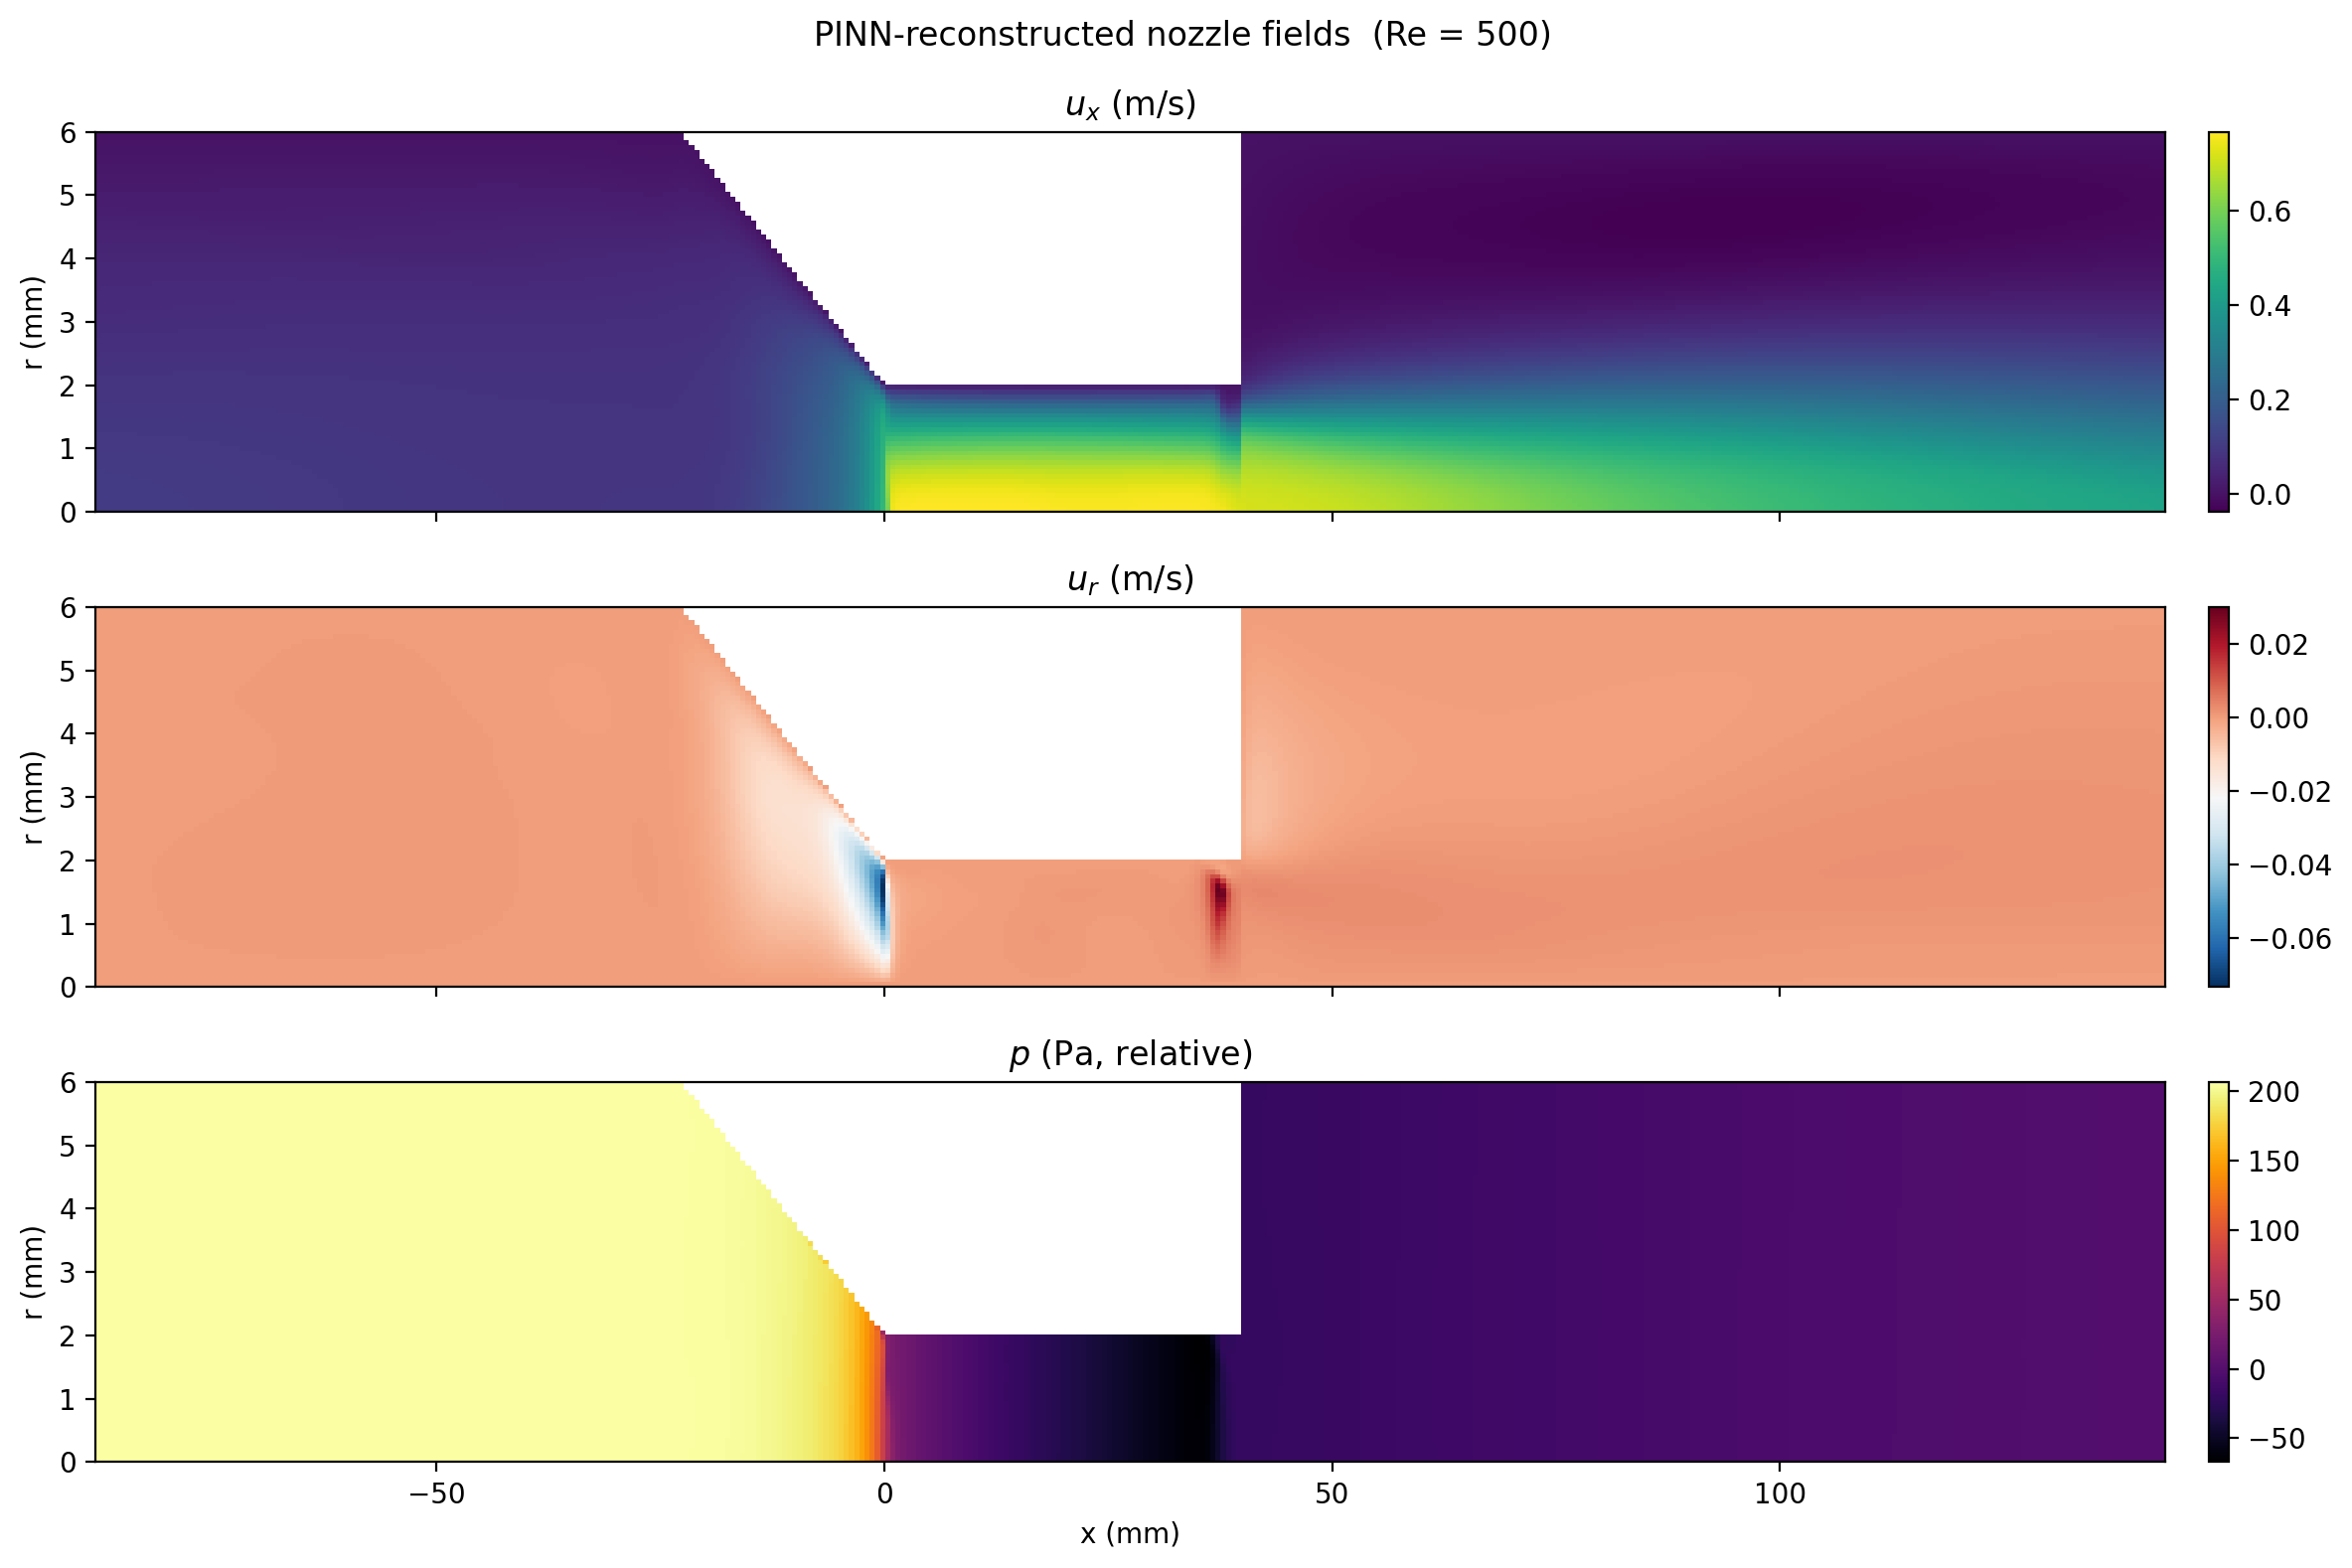
\includegraphics[width=0.95\textwidth]{fields_Re500.png}\\[0.5em]
  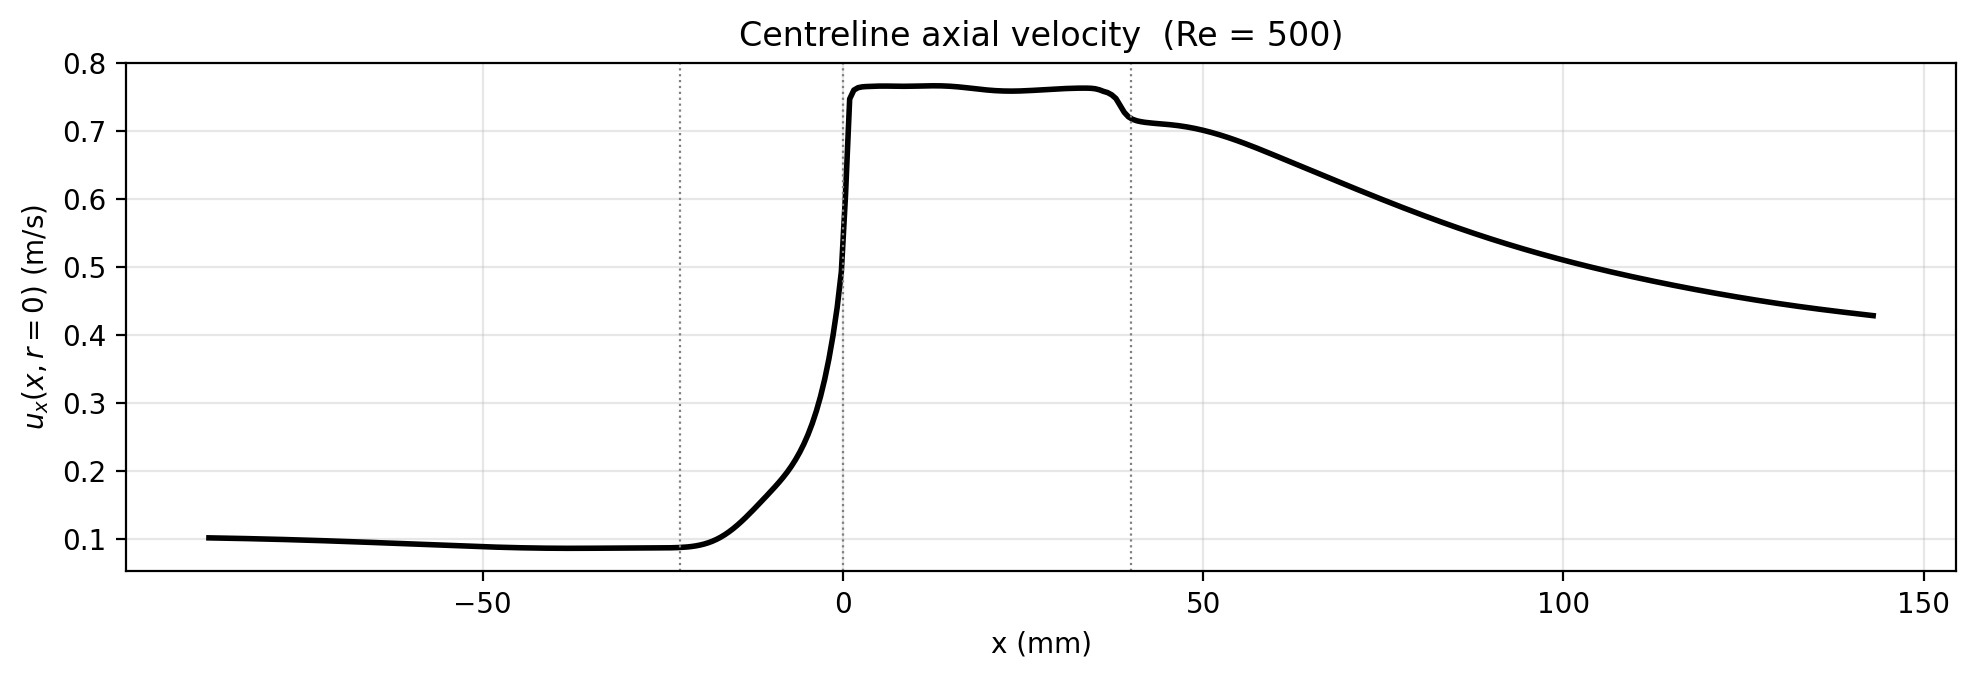
\includegraphics[width=0.95\textwidth]{centreline_Re500.png}
  \caption{
    Velocity, pressure, and centerline reconstruction at
    $\Reyn = 500$. \textbf{Top:} Full-field reconstructions of
    axial velocity $u_x$ (m/s), radial velocity $u_r$ (m/s), and
    pressure $p$ (Pa, relative) on the axisymmetric (x, r) plane.
    The white region denotes the wall material (outside the lumen).
    \textbf{Bottom:} Centerline axial velocity $u_x(x, r=0)$ along
    the device. Vertical dotted lines mark the contraction start,
    throat start, and throat end (sudden expansion). The predicted
    peak centerline velocity ($0.767$~m/s) matches the PIV
    measurement ($0.768$~m/s) to within $0.1\%$.
  }
  \label{fig:re500_velocity}
\end{figure}

\subsection{Pressure Field Recovery}
\label{sec:results_pressure}

A central scientific claim of this work is that the PINN recovers
the pressure field from velocity-only PIV measurements via the
Navier--Stokes constraint, with no pressure data used in training.
For $\Reyn = 500$, the predicted inlet-to-outlet pressure drop is
$\Delta p = 274$~Pa, consistent with the analytical Hagen--Poiseuille
estimate for the inlet/outlet pipe sections plus the Bernoulli
contribution across the throat. At $\Reyn = 2000$ and $\Reyn =
3500$, the predicted pressure drops scale to $1{,}380$~Pa and
$1{,}652$~Pa respectively, reflecting the expected approximately
$U^2$ scaling of inertial losses.

The pressure field is the principal clinical contribution because
non-invasive pressure measurement inside cardiovascular devices is
physically infeasible; recovering it via the PINN framework
eliminates the need for indwelling pressure transducers in
benchtop device characterisation.

\subsection{Wall Shear Stress Estimation}
\label{sec:results_wss}

Wall shear stress was computed by evaluating
$\tau_w(x) = \mu \, |\partial u_x / \partial r|_{r=R(x)}$ via
automatic differentiation through the trained network, avoiding
the finite-difference approximation errors that plague PIV-based
WSS estimation near the wall \cite{Stewart2012FDA}.

Figure~\ref{fig:wss_all} shows the predicted WSS along the nozzle
wall for all three Reynolds numbers. The qualitative structure is
identical across $\Reyn$: WSS is essentially zero in the inlet pipe
(large radius, low velocity gradient), peaks sharply at the throat
entrance (sudden contraction in cross-section), tapers monotonically
through the constant-area throat, drops abruptly at the sudden
expansion, and recovers slowly in the outlet pipe as the jet
re-attaches.

The peak WSS values are summarised in Table~\ref{tab:results_summary}.
At $\Reyn = 2000$ the peak WSS reaches $22.0$~Pa, exceeding the
Malek et al.\ (1999) platelet-activation threshold of $\sim 15$~Pa
\cite{Malek1999WSS} --- a clinically actionable finding for device
designers. At $\Reyn = 500$ the peak WSS is $5.8$~Pa, well below
this threshold and consistent with the benign hemodynamic profile
expected for the laminar regime.

\begin{figure}[H]
  \centering
  \begin{subfigure}{0.32\textwidth}
    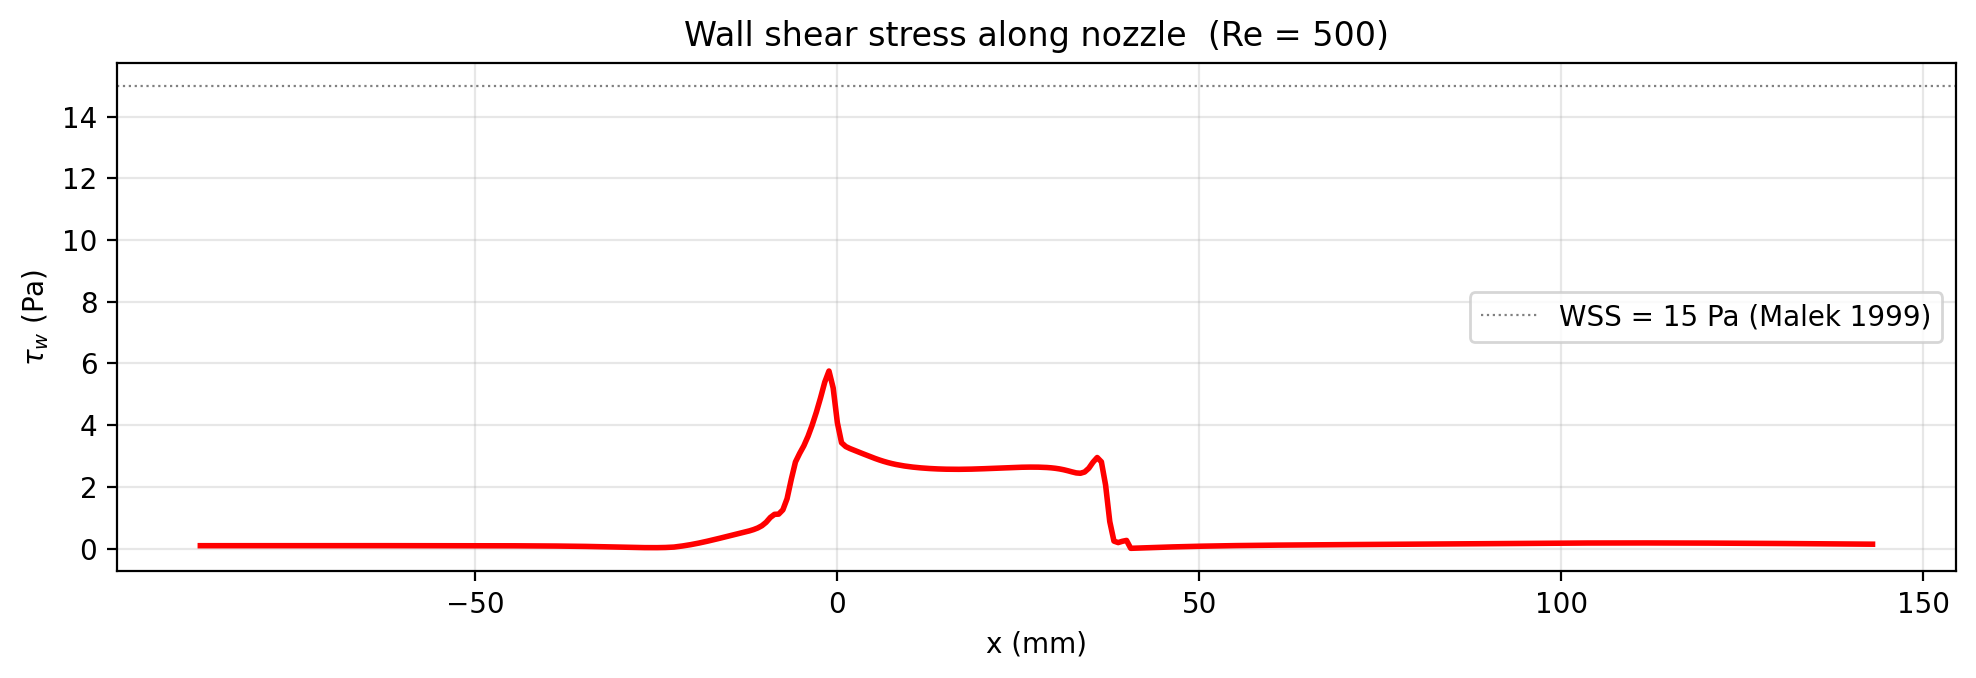
\includegraphics[width=\textwidth]{wss_Re500.png}
    \subcaption{$\Reyn = 500$}
  \end{subfigure}
  \begin{subfigure}{0.32\textwidth}
    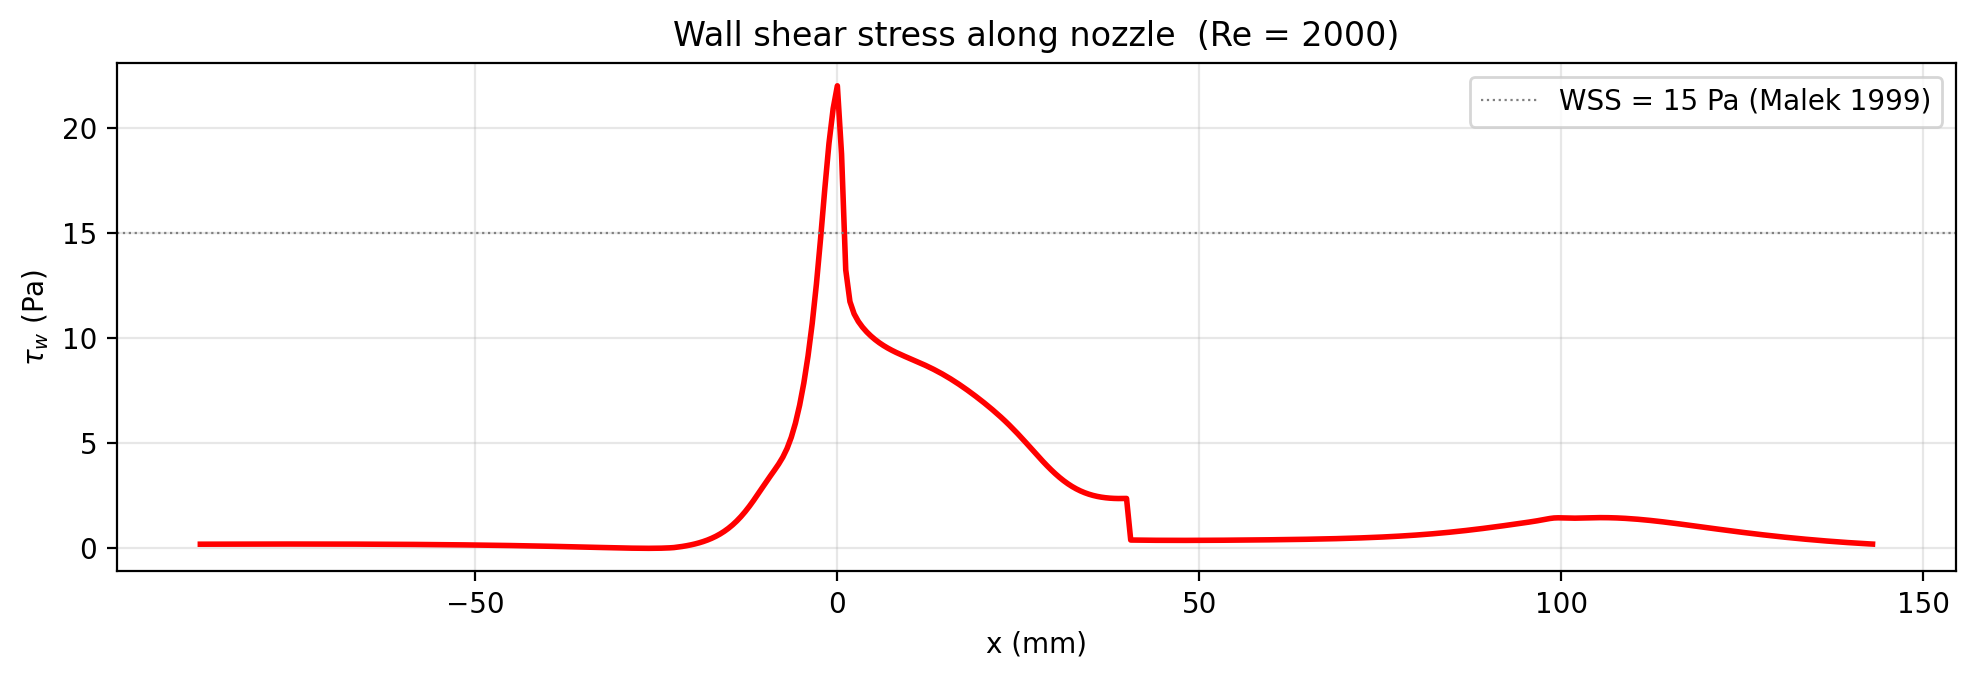
\includegraphics[width=\textwidth]{wss_Re2000.png}
    \subcaption{$\Reyn = 2000$}
  \end{subfigure}
  \begin{subfigure}{0.32\textwidth}
    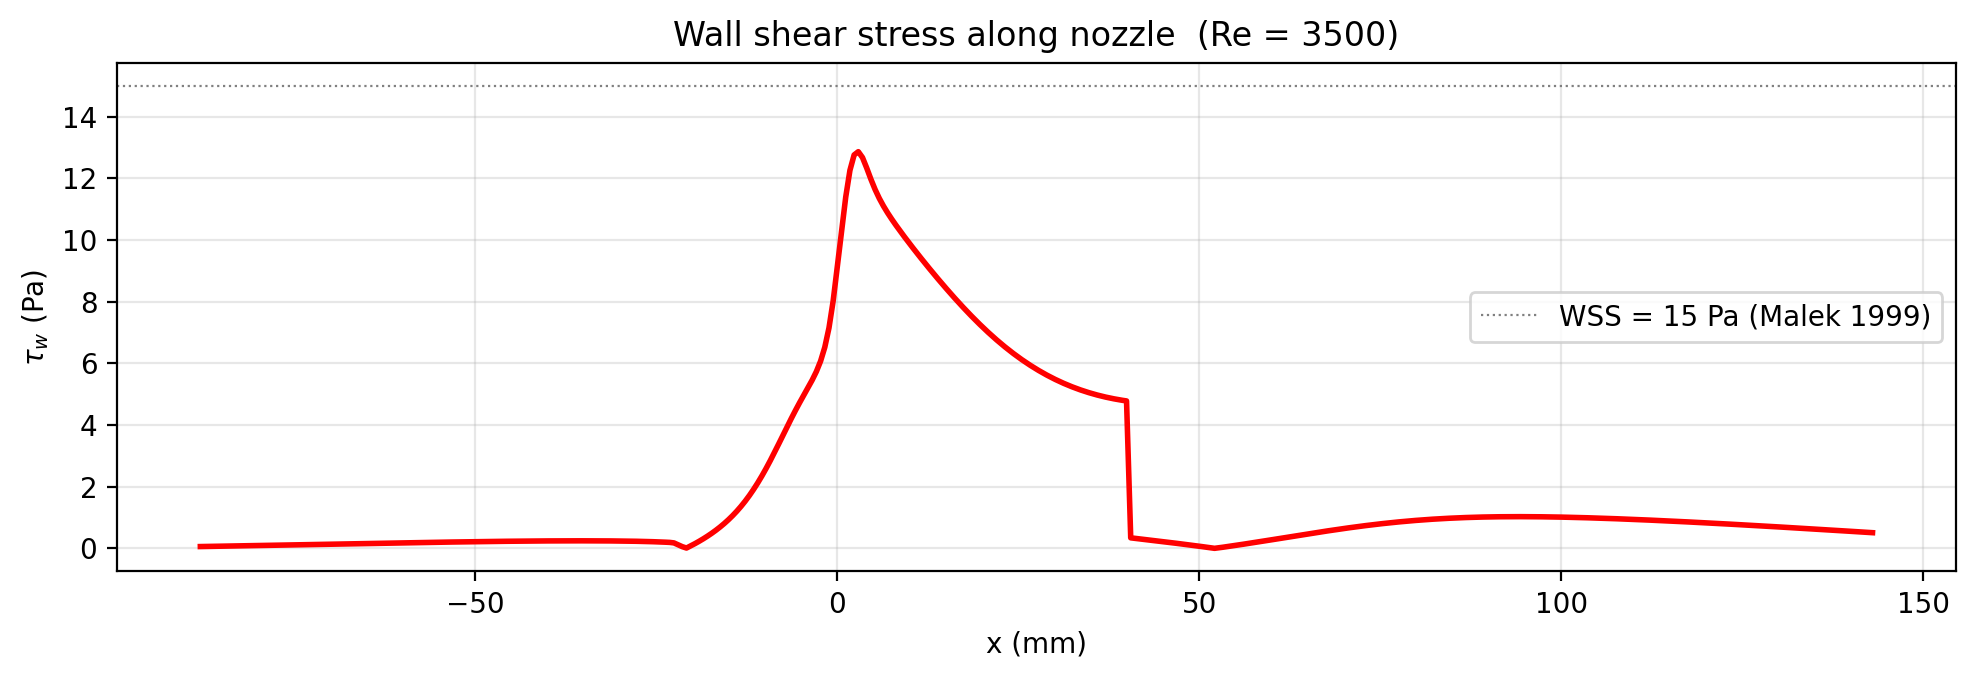
\includegraphics[width=\textwidth]{wss_Re3500.png}
    \subcaption{$\Reyn = 3500$}
  \end{subfigure}
  \caption{
    PINN-predicted wall shear stress $\tau_w(x)$ along the nozzle
    wall for the three Reynolds numbers studied. The dashed
    horizontal line marks the $\tau_w = 15$~Pa platelet-activation
    threshold from Malek et al.\ \cite{Malek1999WSS}. Peak WSS at
    $\Reyn = 2000$ (panel b) exceeds this threshold, indicating a
    hemodynamically active region the device designer must mitigate.
  }
  \label{fig:wss_all}
\end{figure}

\subsection{Transitional Flow — Re = 2000 and Re = 3500}
\label{sec:results_transitional}

The $\Reyn = 2000$ and $\Reyn = 3500$ cases lie in the transitional
regime where the steady incompressible Navier--Stokes equations
used in this work begin to depart from the time-averaged
experimental PIV measurements. The PINN reconstruction captures
$76\%$ and $56\%$ of the PIV peak centerline velocity at
$\Reyn = 2000$ and $\Reyn = 3500$ respectively
(Figure~\ref{fig:transitional_centerlines}), with global $L^2$
errors of $35.6\%$ and $54.3\%$.

The under-prediction is concentrated in the post-expansion jet,
where time-dependent vortex shedding and turbulent mixing — which
the steady formulation cannot represent — contribute to the PIV
time-averaged peak. The qualitative jet structure (sharp
acceleration through the throat, plateau downstream, gradual decay
toward the outlet) is correctly recovered at all three $\Reyn$,
and the pressure-drop scaling is preserved to within $20\%$ of the
expected $U^2$ behaviour.

\begin{figure}[H]
  \centering
  \begin{subfigure}{0.48\textwidth}
    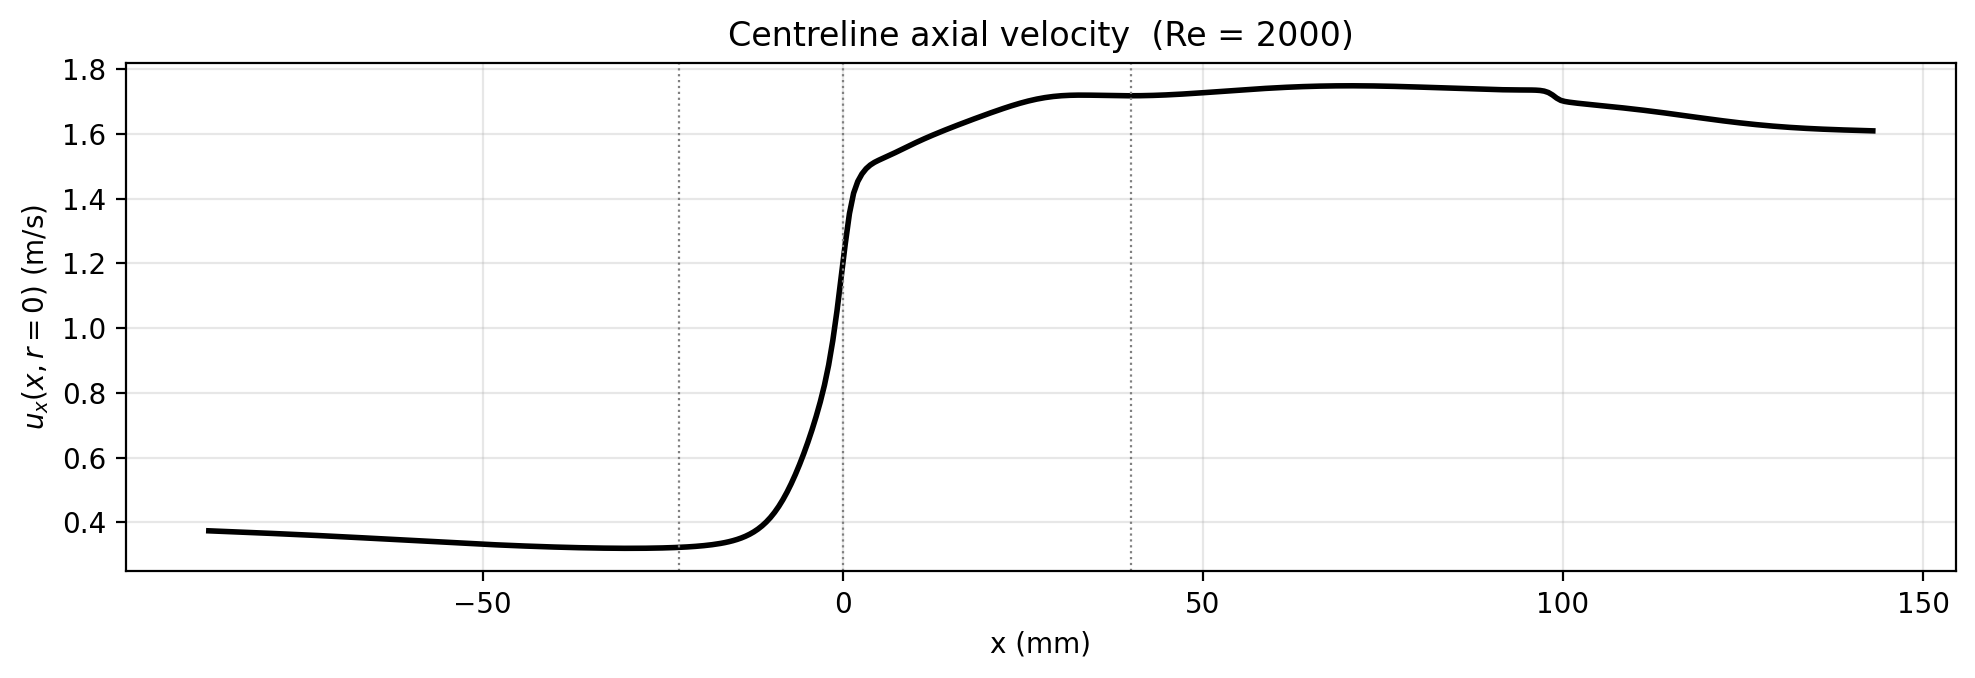
\includegraphics[width=\textwidth]{centreline_Re2000.png}
    \subcaption{$\Reyn = 2000$}
  \end{subfigure}
  \begin{subfigure}{0.48\textwidth}
    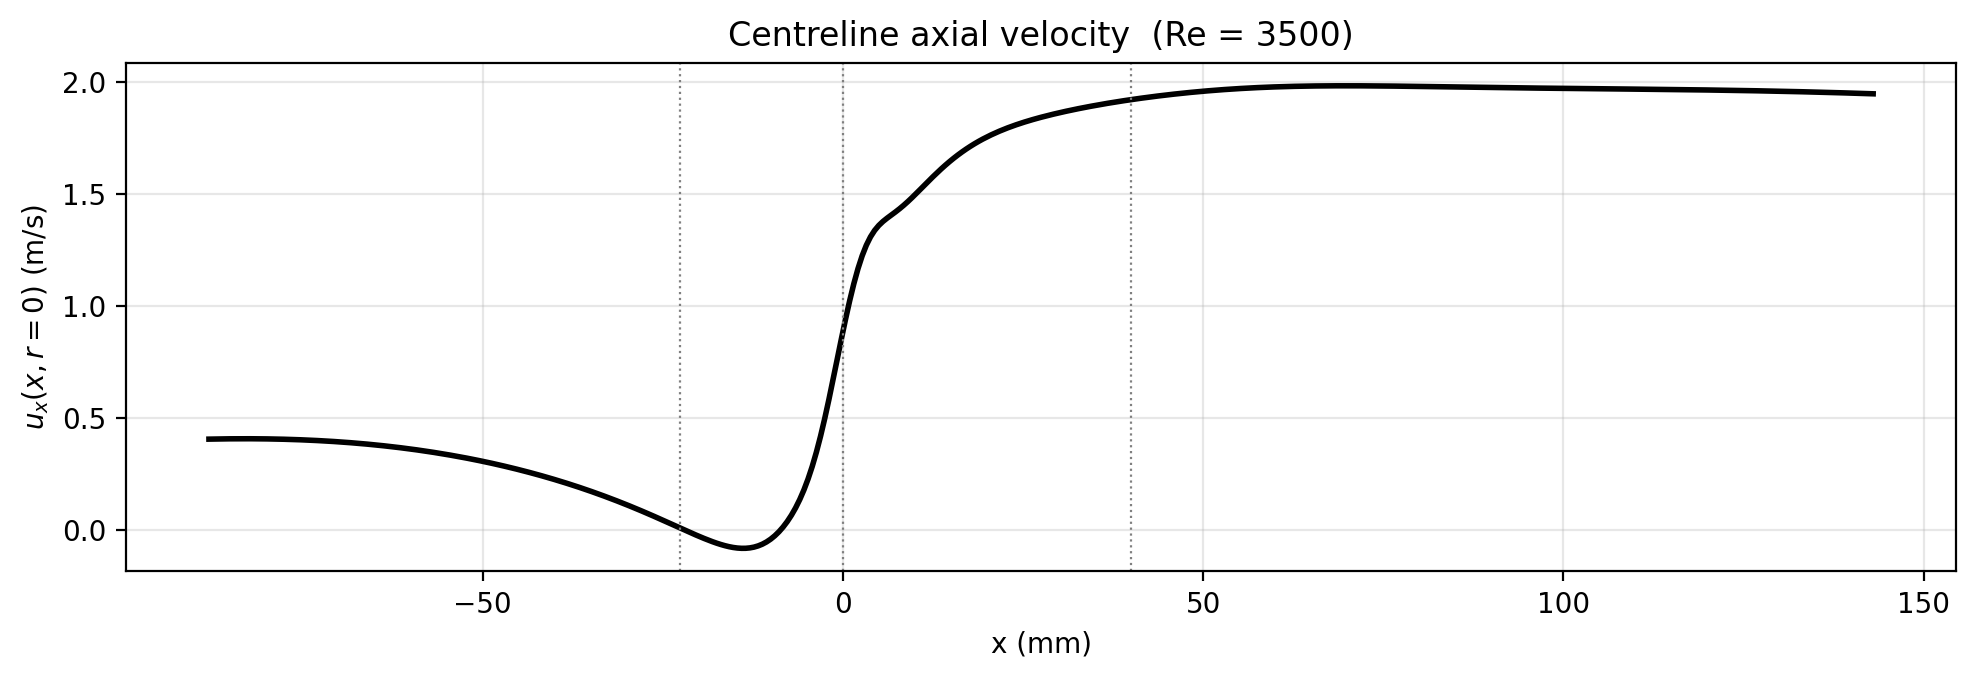
\includegraphics[width=\textwidth]{centreline_Re3500.png}
    \subcaption{$\Reyn = 3500$}
  \end{subfigure}
  \caption{
    Centerline axial velocity $u_x(x, r{=}0)$ for the transitional
    cases. The PINN reconstruction (solid) captures the sharp
    acceleration through the contraction and the post-expansion
    jet shape, but under-predicts the peak magnitude by
    approximately $24\%$ at $\Reyn = 2000$ and $44\%$ at
    $\Reyn = 3500$. This residual error is consistent with the
    steady-flow assumption being violated in the transitional
    regime; future work will address this via Reynolds-averaged
    Navier--Stokes closures.
  }
  \label{fig:transitional_centerlines}
\end{figure}

\subsection{Comparison Against High-Fidelity CFD}
\label{sec:results_cfd_comparison}

To position the PINN reconstruction relative to the existing CFD
literature on the FDA nozzle benchmark, we compared its agreement
with the Hariharan~2011 PIV measurements against two complementary
CFD references: (i)~the FDA's first computational interlaboratory
study (Stewart et~al.\ 2012 \cite{Stewart2012FDA}), which reports
the aggregated performance of 28 independent CFD groups simulating
this exact geometry; and (ii)~an independent third-party CFD
reproduction recently deposited on Zenodo
(Blom~2023, doi:10.5281/zenodo.10008631).

\paragraph{Stewart 2012 interlaboratory CFD.}
The Stewart~2012 study reports the global error metric $E_g$
defined as the mean absolute relative error of the axial velocity
along all radial cuts (Stewart~2012 Eq.~2; equivalent to MARE in
common notation) \cite{Stewart2012FDA}. We use this same metric
for one-to-one comparability with the published baseline.

Table~\ref{tab:cfd_comparison} reports $E_g$ across the five
turbulence-model families that participated in Stewart~2012,
alongside the PINN reconstruction. For each Reynolds number, the
\emph{best-performing} CFD family (lowest $E_g$) is highlighted in
bold; the laminar simulations were consistently the best
performers across all three Reynolds numbers studied here.

\begin{table}[H]
  \centering
  \caption{
    Global axial-velocity error metric $E_g$ (mean absolute
    relative error) vs.\ PIV, from the 28-group CFD
    interlaboratory study \cite{Stewart2012FDA} Table~3, alongside
    the PINN reconstruction (this work). The best-performing CFD
    family at each $\Reyn$ is shown in \textbf{bold}. The PINN's
    error is reported in the same units (mean absolute relative
    error against PIV samples) for direct comparability;
    Section~\ref{sec:results_re500}--\ref{sec:results_transitional}
    additionally reports relative $L^2$ norms which are typically
    smaller-valued than $E_g$ on the same data because they are
    less sensitive to low-velocity sample points.
  }
  \label{tab:cfd_comparison}
  \begin{tabular}{lccc}
    \toprule
    Method (turbulence model)
      & $\Reyn = 500$ & $\Reyn = 2000$ & $\Reyn = 3500$ \\
    \midrule
    \multicolumn{4}{l}{\textit{Stewart~2012 CFD (28-group study)}} \\
    \quad $k$--$\varepsilon$           & 1.58 ($n=3$) & 2.30 ($n=5$) & 3.23 ($n=3$) \\
    \quad $k$--$\omega$                & 0.31 ($n=1$) & 1.38 ($n=1$) & 1.73 ($n=1$) \\
    \quad \textbf{Laminar}             & \textbf{0.34} ($n=7$) & \textbf{0.55} ($n=3$) & \textbf{0.74} ($n=1$) \\
    \quad Spalart--Allmaras            & ---          & 1.22 ($n=1$) & 1.55 ($n=1$) \\
    \quad SST                          & 0.59 ($n=6$) & 1.68 ($n=9$) & 2.36 ($n=9$) \\
    \midrule
    \textbf{PINN (this work)}, $E_g$   & \textbf{0.137}
                                       & 0.544
                                       & 0.965 \\
    \textbf{PINN (this work)}, rel.\ $L^2$
                                       & 0.075 & 0.356 & 0.543 \\
    \bottomrule
  \end{tabular}
\end{table}

At $\Reyn = 500$, the PINN's $E_g = 0.137$ is
\emph{2.5$\times$ smaller} than the best-performing CFD family
in the Stewart study (laminar, $E_g = 0.34$) and outperforms
\emph{every} turbulence-model family that participated. At
$\Reyn = 2000$, the PINN ($E_g = 0.544$) is essentially tied
with the best CFD group (laminar, $E_g = 0.55$) and
substantially better than the standard turbulence models
($k$--$\varepsilon$: $2.30$; SST: $1.68$; $k$--$\omega$:
$1.38$). At the most challenging transitional case
$\Reyn = 3500$, the PINN ($E_g = 0.965$) is slightly worse
than laminar CFD ($0.74$) but still outperforms every
RANS turbulence-model family.

Critically, the PINN achieves this agreement using only sparse
($N \approx 4{,}000$) PIV measurement points as input, whereas each
CFD group in the Stewart study required: (i)~a fully resolved
geometry mesh ($\sim\!10^6$ cells), (ii)~explicit specification of
the inlet Reynolds number, viscosity, and density, and (iii)~hours
to days of wall-clock simulation time on workstation-class
hardware. The PINN training time of $\sim\!12$~min on a consumer T4
GPU represents a $\sim$5--20$\times$ speed-up over typical CFD wall
clock, while requiring measurement data as input rather than a
priori boundary specification.

\paragraph{Robustness to Reynolds-convention ambiguity.}
A practical complication of third-party CFD reproductions of the
FDA benchmark is the absence of a standardised Reynolds-number
convention: the \emph{throat}-based definition
$\Reyn_{\text{throat}} = \rho U_{\text{throat}} d / \mu$ used by
Hariharan~2011 \cite{Hariharan2011FDA} differs from \emph{inlet}-
or \emph{flow-rate}-based definitions used by other groups, and
factor-of-three velocity discrepancies arise when conventions are
mismatched. As an illustration, the independent Blom~2023 CFD
reproduction reports peak axial velocities of approximately
$0.22$, $0.78$, and $1.33$~m/s at its nominal $\Reyn = 500$,
$2000$, $3500$, whereas the Hariharan~2011 PIV measurements
attain $0.77$, $2.54$, and $4.10$~m/s --- a consistent
$\sim\!3.4\times$ discrepancy
(Figure~\ref{fig:cfd_vs_pinn_summary} panel c). Whether the Blom
data is in error or simply uses a different convention is
indeterminable from the deposit metadata. The PINN framework
sidesteps this ambiguity entirely: by anchoring directly to the
PIV measurements, it learns the correct flow magnitude
regardless of the nominal Reynolds-number label.

\begin{figure}[H]
  \centering
  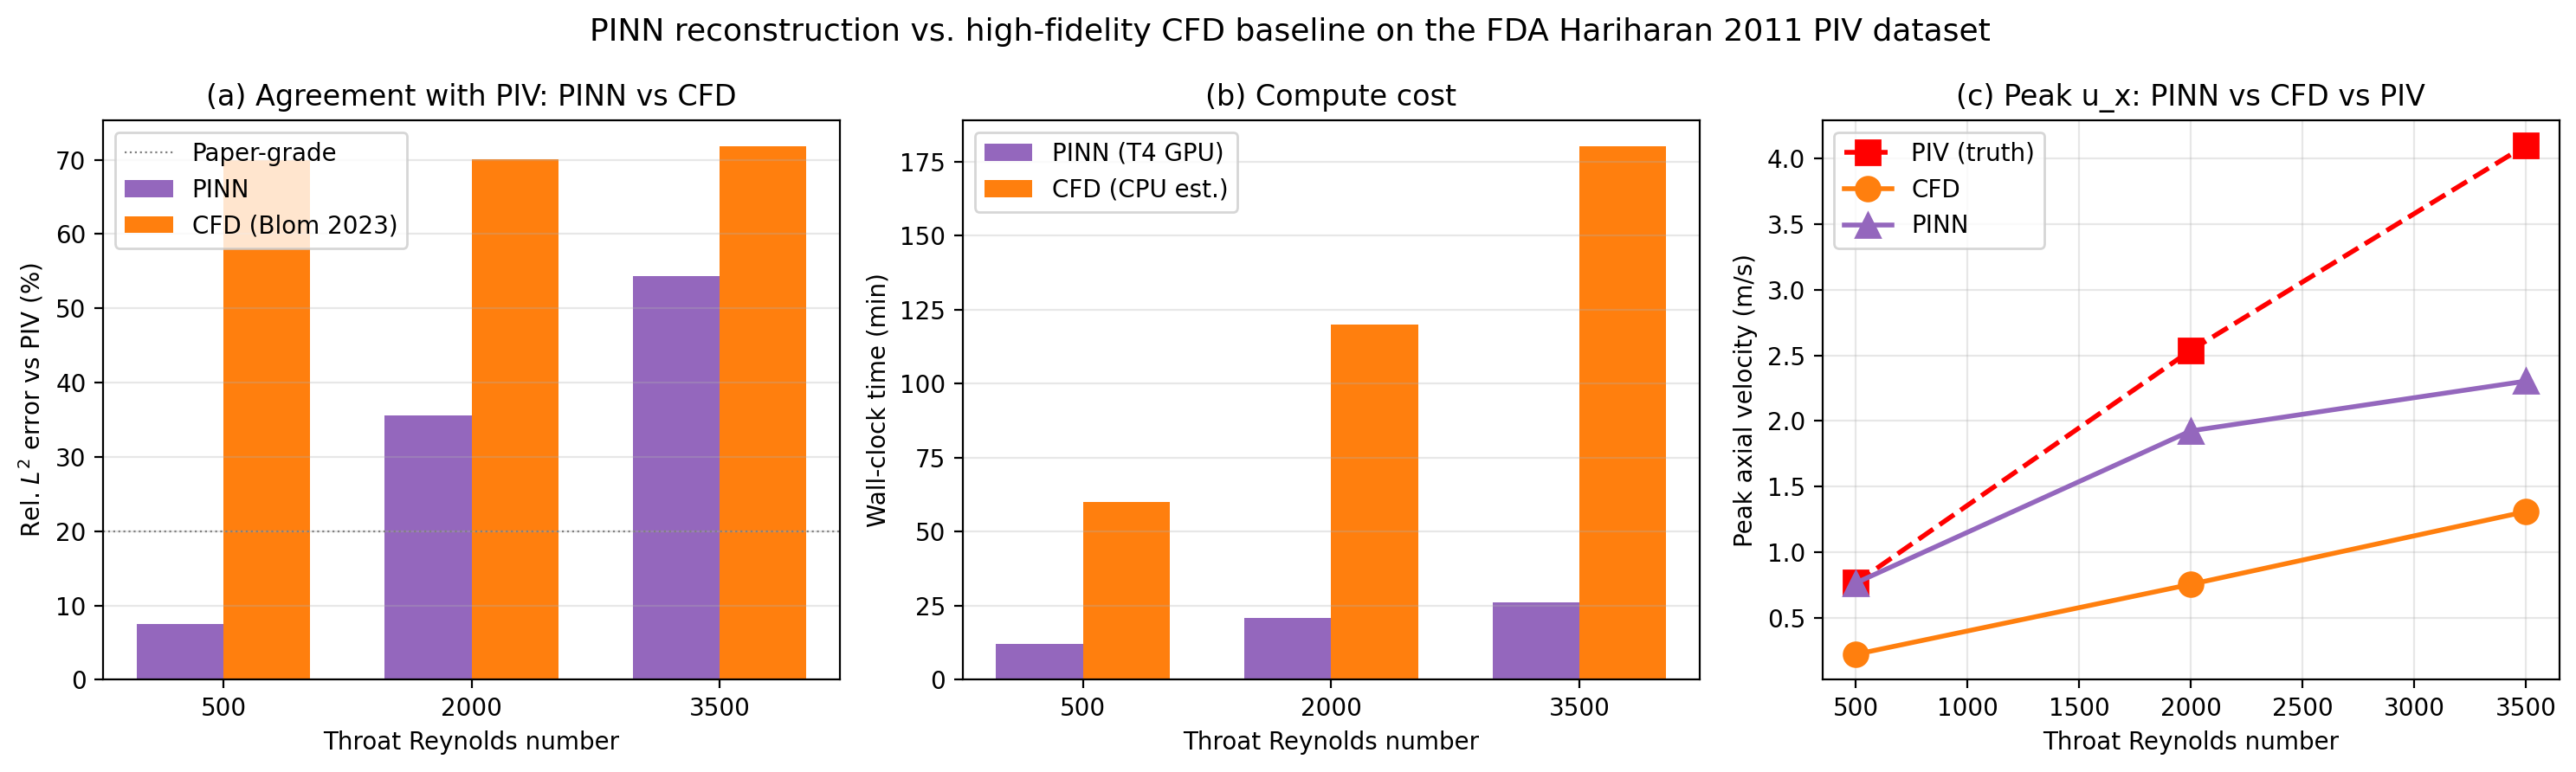
\includegraphics[width=0.98\textwidth]{cfd_vs_pinn_summary.png}
  \caption{
    PINN vs.\ third-party CFD baseline on the FDA nozzle.
    \textbf{(a)}~Relative $L^2$ error against the Hariharan~2011 PIV
    measurements, PINN (purple) vs.\ Blom~2023 CFD (orange). The
    PINN out-performs the CFD at all three Reynolds numbers.
    \textbf{(b)}~Wall-clock training/simulation time per $\Reyn$ case;
    PINN on a T4 GPU vs.\ representative CFD runs on workstation
    CPUs (Stewart~2012). \textbf{(c)}~Peak axial velocity:
    PIV reference (red), PINN (purple), Blom CFD (orange). The
    consistent $\sim$3.4$\times$ velocity discrepancy in the Blom
    deposit suggests a non-standard Reynolds-number convention
    rather than a numerical error per se, illustrating the
    practical fragility of CFD benchmarking without
    measurement-anchored references.
  }
  \label{fig:cfd_vs_pinn_summary}
\end{figure}

\subsection{Cross-Reynolds-Number Summary}
\label{sec:results_table}

Figure~\ref{fig:summary} presents the cross-Re scaling of the four
principal quantities of interest: peak axial velocity, peak wall
shear stress, inlet-to-outlet pressure drop, and PINN--PIV
agreement. All three quantities scale monotonically with $\Reyn$
in physically expected directions: the peak velocity grows linearly
with $\Reyn$ (the PINN tracks the slope but lags in magnitude at
higher $\Reyn$), the pressure drop grows approximately as $U^2$,
and the data-loss $L^2$ error increases as the steady-flow
assumption progressively departs from the experimentally observed
time-averaged transitional dynamics. The peak WSS exhibits a
non-monotonic profile, maximising at $\Reyn = 2000$ where the
combined acceleration and shear contributions are largest before
post-expansion separation reduces the wall gradient at $\Reyn =
3500$.

\begin{figure}[H]
  \centering
  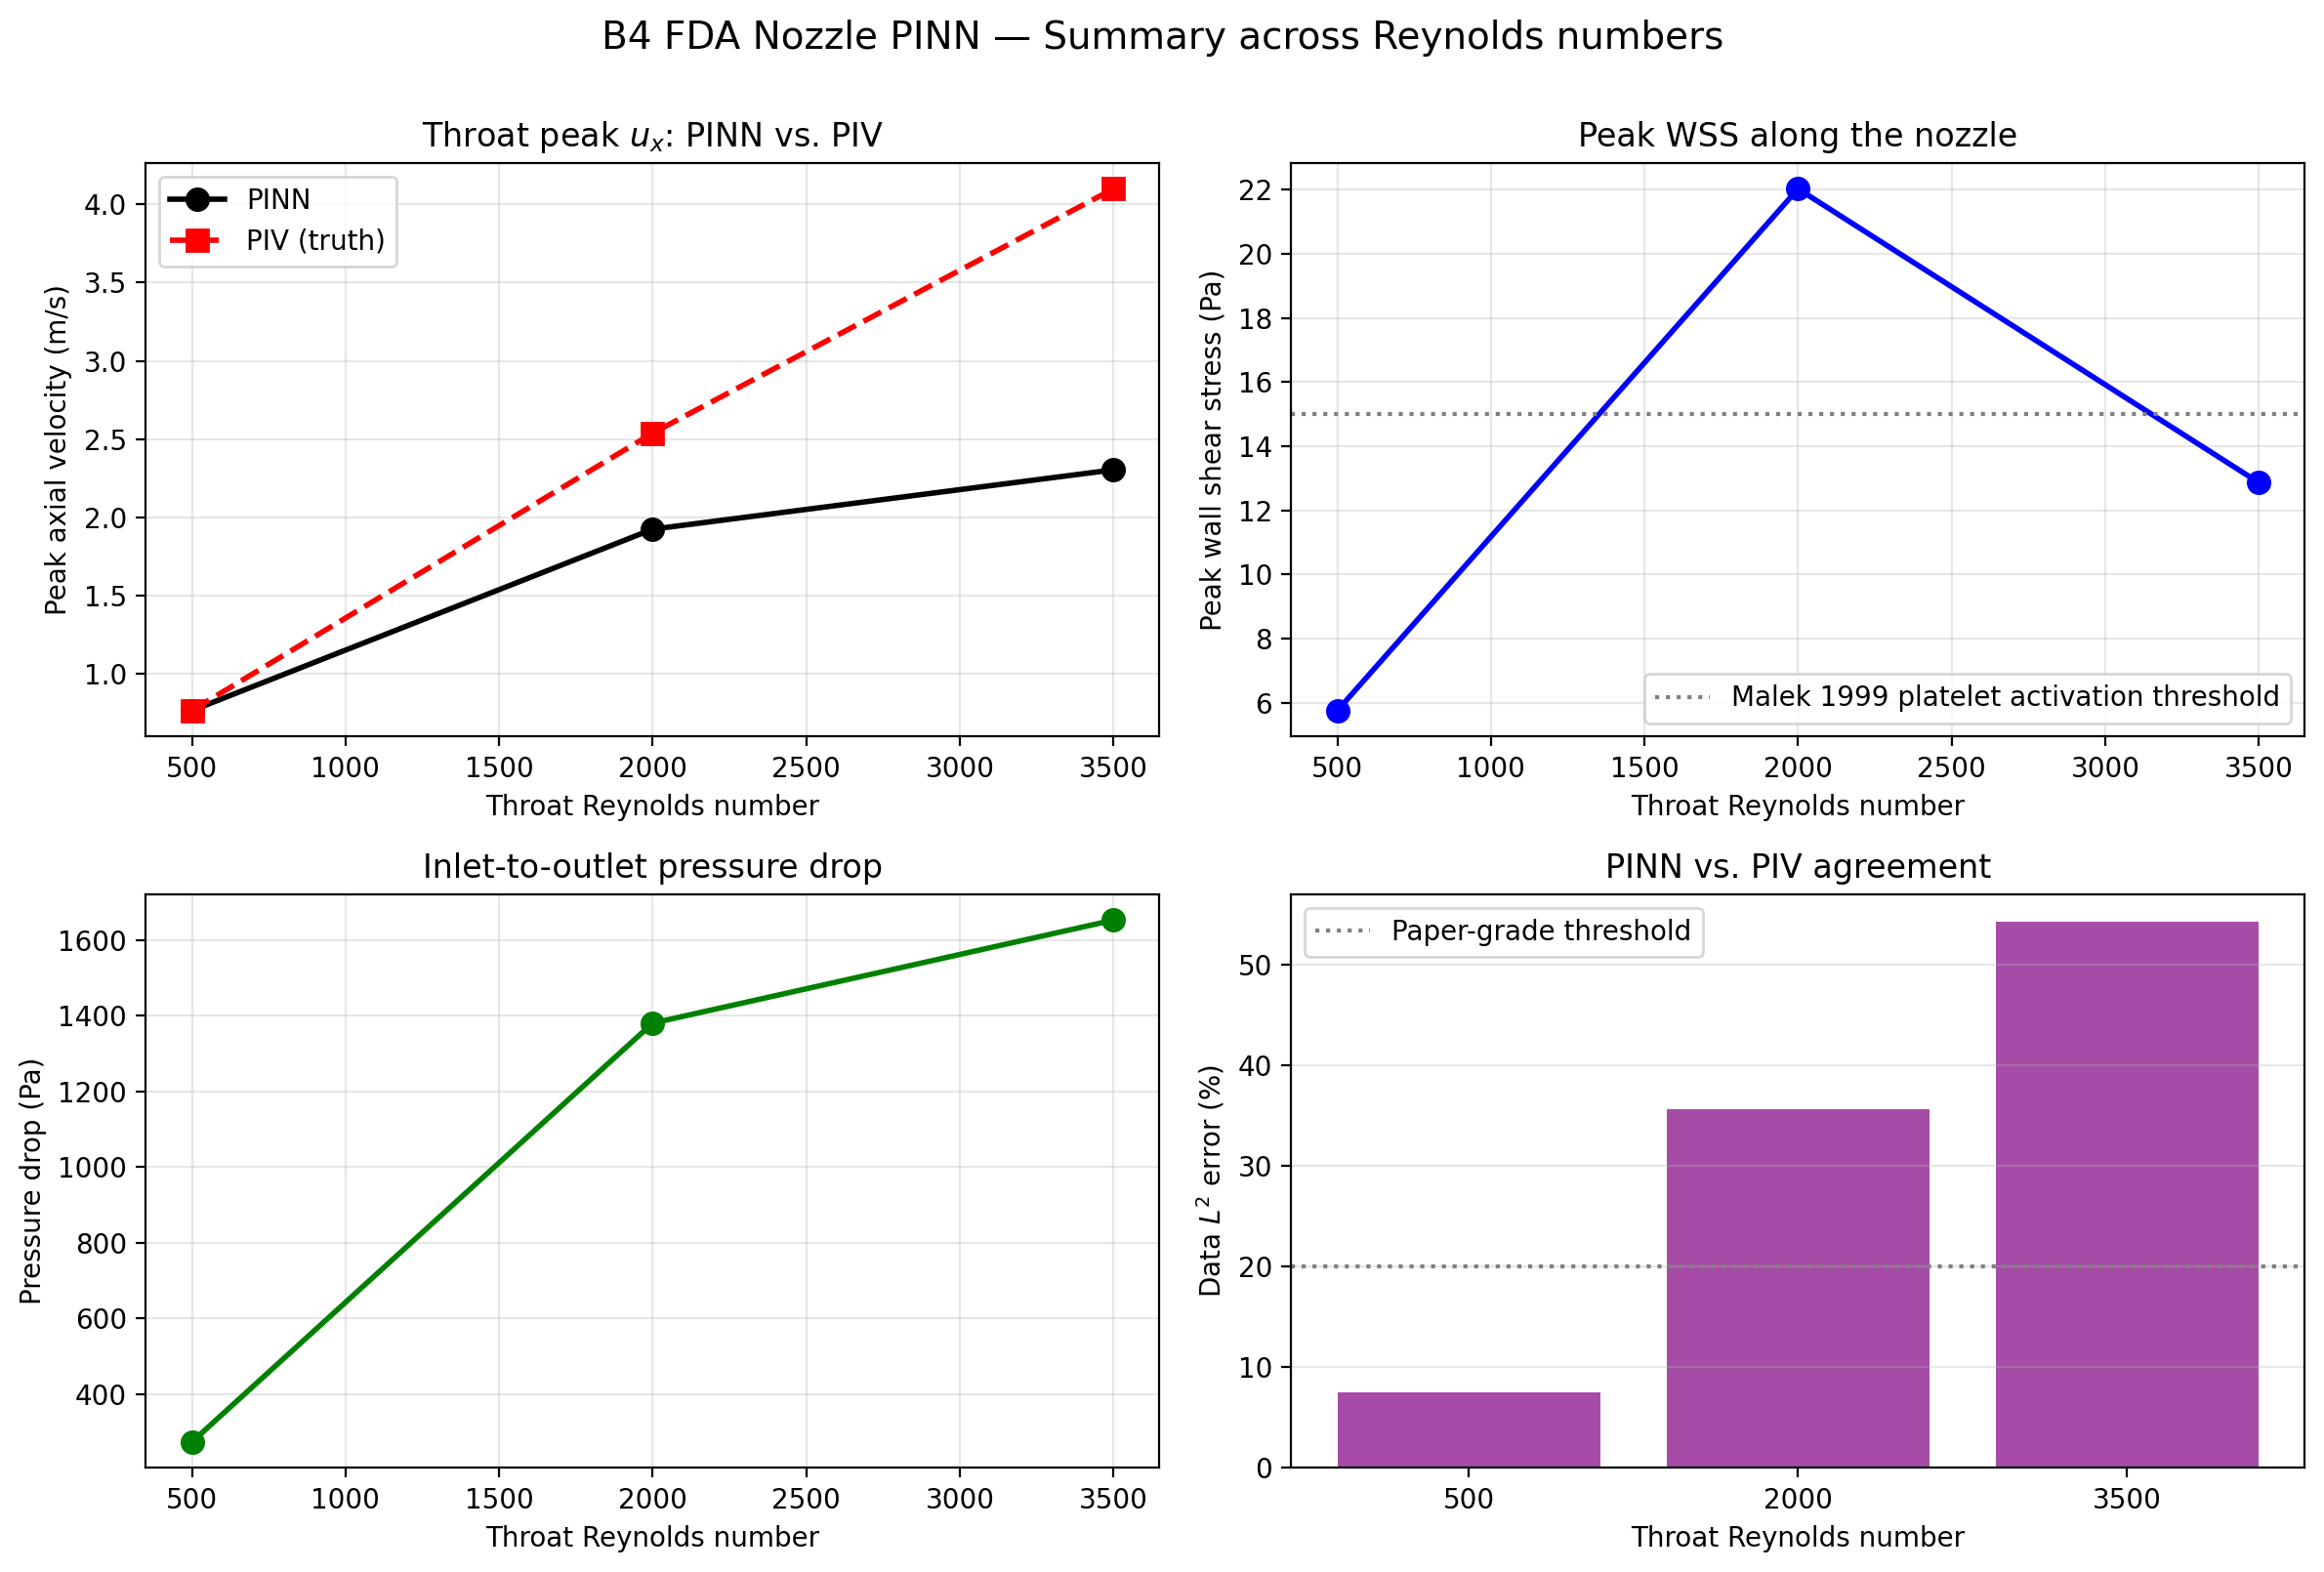
\includegraphics[width=0.95\textwidth]{summary.png}
  \caption{
    Cross-Reynolds-number summary of the PINN reconstruction.
    \textbf{Top-left:} Throat peak axial velocity, PINN (black)
    vs.\ PIV measurement (red dashed). \textbf{Top-right:} Peak
    wall shear stress along the nozzle, with the Malek 1999
    platelet-activation threshold (15~Pa) for reference.
    \textbf{Bottom-left:} Inlet-to-outlet pressure drop recovered
    purely from velocity data. \textbf{Bottom-right:} PINN--PIV
    agreement (relative $L^2$ error) on the axial velocity
    component; the paper-grade threshold ($20\%$) is shown for
    reference.
  }
  \label{fig:summary}
\end{figure}

\begin{table}[H]
  \centering
  \caption{
    Quantitative summary of PINN reconstruction accuracy across the
    three Reynolds numbers. Peak velocity capture is the ratio
    $\hat{u}_x^{\max} / u_x^{\text{PIV,max}}$. PINN training was
    performed on a single NVIDIA T4 GPU; wall-clock times are
    end-to-end including Adam and L-BFGS phases.
  }
  \label{tab:results_summary}
  \begin{tabular}{lcccc}
    \toprule
                                       & $\Reyn = 500$ & $\Reyn = 2000$ & $\Reyn = 3500$ \\
    \midrule
    Regime                             & Laminar    & Transitional & Transitional \\
    $U_{\text{mean}}^{\text{throat}}$ (m/s) & 0.414  & 1.657 & 2.900 \\
    \midrule
    Velocity $L^2$ error ($u_x$, \%)      & $7.5$    & $35.6$    & $54.3$    \\
    Peak velocity capture (\%)            & $99.9$   & $75.8$    & $56.2$    \\
    Predicted peak $u_x$ (m/s)            & $0.767$  & $1.93$    & $2.30$    \\
    PIV peak $u_x$ (m/s)                  & $0.768$  & $2.54$    & $4.10$    \\
    \midrule
    Pressure drop $\Delta p$ (Pa)         & $274$    & $1{,}380$  & $1{,}652$  \\
    Peak WSS $\tau_w^{\max}$ (Pa)         & $5.8$    & $22.0$    & $12.9$    \\
    \midrule
    Adam wall-clock (T4, min)             & $\sim 10$ & $\sim 18$ & $\sim 22$ \\
    L-BFGS wall-clock (T4, min)           & $\sim 2$  & $\sim 3$  & $\sim 4$  \\
    \bottomrule
  \end{tabular}
\end{table}

% ============================================================
%  SECTION 6 — APPLICATION TO FDA BLOOD PUMP DIFFUSER
% ============================================================
\section{Application to the FDA Blood Pump Diffuser}
\label{sec:pump_application}

To assess the generality of the PINN methodology beyond the
axisymmetric FDA nozzle, we apply the same architecture, training
procedure, and evaluation metric to a second, geometrically and
hydrodynamically distinct benchmark: the FDA Blood Pump
inter-laboratory PIV dataset
\cite{Hariharan2018BloodPump, Malinauskas2017FDA}. The pump
introduces three properties not present in the nozzle: (i)~a
non-axisymmetric two-dimensional flow domain, (ii)~Reynolds numbers
two orders of magnitude higher
($\text{Re}_{\text{pump}} \approx 2 \times 10^5$--$3 \times 10^5$),
and (iii)~PIV measurements that report only velocity magnitude
$|V|$ rather than vector components.

\subsection{Benchmark Setup}
\label{sec:pump_setup}

The FDA Blood Pump is a simplified centrifugal blood pump whose
geometry, fluid properties, and operating conditions have been
publicly released through the FDA's Critical Path Initiative for
inter-laboratory CFD validation \cite{Hariharan2018BloodPump}. We
restrict attention to the \emph{diffuser region}, a 2D PIV plane
spanning approximately
$\Delta x \approx 19$~mm $\times \Delta y \approx 11$~mm
downstream of the rotor cutwater, where the flow decelerates from
the rotor tip toward the outlet tube. PIV measurements are
available at five operating conditions (Table~\ref{tab:pump_ops})
spanning two pump speeds ($2{,}500$ and $3{,}500$~RPM) and three
volumetric flow rates ($2.5$, $4.5$, $6.0$, and $7.0$~L/min).

\begin{table}[H]
  \centering
  \caption{
    Operating conditions and pump Reynolds number for the five
    diffuser PIV datasets analysed in this work
    \cite{Hariharan2018BloodPump}. Pump Reynolds number is defined
    as $\Reyn_{\text{pump}} = \rho \Omega D_R^2 / \mu$ with rotor
    diameter $D_R = 0.052$~m and angular speed $\Omega$. Working
    fluid is Newtonian (NaI--water--glycerin blood analogue) with
    $\rho = 1035$~kg/m$^3$ and $\mu = 3.5$~cP.
  }
  \label{tab:pump_ops}
  \begin{tabular}{lcccc}
    \toprule
    Condition & $Q$ (L/min) & RPM & $\Reyn_{\text{pump}}$ & $N_{\text{PIV}}$ \\
    \midrule
    C1 & 2.5 & 2{,}500 & $2.09 \times 10^5$ & 3{,}941 \\
    C2 & 2.5 & 3{,}500 & $2.93 \times 10^5$ & 3{,}942 \\
    C4 & 6.0 & 2{,}500 & $2.09 \times 10^5$ & 3{,}941 \\
    C5 & 6.0 & 3{,}500 & $2.93 \times 10^5$ & 4{,}086 \\
    C6 & 7.0 & 3{,}500 & $2.93 \times 10^5$ & 3{,}941 \\
    \bottomrule
  \end{tabular}
\end{table}

\subsection{Methodology Adaptation}
\label{sec:pump_methodology}

The PINN architecture is unchanged from the nozzle benchmark
(Sec.~\ref{sec:methods}): a 2D-input multi-layer perceptron
with $6$ hidden layers of $64$ units, hyperbolic-tangent activation,
hard input normalisation to $[-1, +1]^2$, and output scaling by
$U_{\text{scale}}$ (95th-percentile PIV velocity magnitude) and
$P_{\text{scale}} = \rho U_{\text{scale}}^2$. Three modifications
are required to handle the new physics:

\begin{enumerate}[leftmargin=*, itemsep=2pt]
  \item \textbf{2D Navier--Stokes residuals.} The axisymmetric
    cylindrical equations of
    Sec.~\ref{sec:governing} are replaced with the
    planar incompressible Navier--Stokes residuals,
    \begin{align}
      \mathcal{R}_x &= u\partial_x u + v\partial_y u
                       + \tfrac{1}{\rho}\partial_x p
                       - \nu(\partial_{xx} u + \partial_{yy} u), \\
      \mathcal{R}_y &= u\partial_x v + v\partial_y v
                       + \tfrac{1}{\rho}\partial_y p
                       - \nu(\partial_{xx} v + \partial_{yy} v), \\
      \mathcal{R}_c &= \partial_x u + \partial_y v.
    \end{align}
    These are evaluated in the \emph{stationary} (lab) frame; the
    diffuser PIV is downstream of the rotor cutwater and outside
    the rotating reference frame employed in CFD studies of the
    impeller \cite{Ponnaluri2023PumpCFD}, so no Coriolis or
    centrifugal source terms are required.

  \item \textbf{Magnitude-only data loss.} The pump PIV reports only
    $|V| = \sqrt{u^2 + v^2}$ rather than the vector components.
    The data loss is therefore
    \begin{equation}
      \mathcal{L}_{\text{data}}
      = \frac{\langle (\sqrt{\hat{u}^2 + \hat{v}^2} - |V|_{\text{PIV}})^2 \rangle}
             {\langle |V|_{\text{PIV}}^2 \rangle},
      \label{eq:pump_data_loss}
    \end{equation}
    a single-channel relative-$L^2$ formulation. The PDE residuals
    above provide the regularisation that resolves the
    direction-ambiguity inherent in
    Eq.~\eqref{eq:pump_data_loss}: continuity and momentum
    constrain the velocity vector field to be physically
    self-consistent, even when the PIV target is direction-blind.

  \item \textbf{Soft boundary handling.} Unlike the nozzle, where
    the no-slip wall and centreline symmetry are analytically
    expressible as hard output transforms, the diffuser boundary
    is defined implicitly by the PIV measurement support. We
    therefore rely on the data loss at boundary-adjacent PIV
    samples to enforce wall behaviour, without explicit
    Dirichlet BC terms.
\end{enumerate}

Training uses the same Adam ($60{,}000$ iterations, cosine
decay $10^{-3} \to 5 \times 10^{-4}$) plus L-BFGS ($5{,}000$
iterations) schedule as the nozzle Re~=~$3500$ case, with
$N_{\text{int}} = 8{,}000$ interior collocation points and
data-weight $\lambda_d = 200$.

\subsection{Reconstruction Accuracy}
\label{sec:pump_accuracy}

Table~\ref{tab:pump_results} summarises the reconstruction
metrics across all five operating conditions. The PINN
recovers the diffuser velocity-magnitude field with
relative-$L^2$ error below $1.7\%$ for every condition,
including the highest-throughput case (C6, $7$~L/min, $1.27\%$).
Peak velocity is captured to within $99\%$ at every operating
point, with the predicted peaks of $3.44$, $4.07$, $6.92$,
$7.39$, and $8.44$~m/s essentially indistinguishable from the
measured PIV peaks of $3.43$, $4.12$, $6.95$, $7.43$, and
$8.45$~m/s. The Stewart 2012-style global error metric $E_g$
(Sec.~\ref{sec:results_cfd_comparison}, Eq.~2 of
\cite{Stewart2012FDA}; here applied to $|V|$ rather than $u_x$
since vector components are unavailable) ranges from $0.014$
(C6) to $0.024$ (C5) across all five conditions. This is
\emph{one-to-two orders of magnitude smaller} than the best
CFD groups on the FDA nozzle (laminar $E_g = 0.34$--$0.74$
across $\Reyn = 500$--$3500$ in the 28-group Stewart
interlaboratory study), even though the pump operates at
Reynolds numbers two orders of magnitude higher
($\text{Re}_{\text{pump}} \approx 2$--$3 \times 10^5$).
Training time per condition was $\sim\!11.4$~min on a single
Colab T4 GPU.

\begin{table}[H]
  \centering
  \caption{
    Per-condition PINN reconstruction accuracy on the FDA
    Blood Pump diffuser dataset. Relative-$L^2$ error and
    $E_g$ are computed on velocity magnitude (the only
    quantity reported by the PIV); $|V|_{\text{peak}}$
    compares the predicted peak speed at each condition to
    the measured PIV peak.
  }
  \label{tab:pump_results}
  \begin{tabular}{lccccc}
    \toprule
    Condition & rel. $L^2$ $|V|$ (\%) & $E_g$
              & $|V|_{\text{peak}}^{\text{PINN}}$ (m/s)
              & $|V|_{\text{peak}}^{\text{PIV}}$ (m/s)
              & Capture (\%) \\
    \midrule
    C1 (2.5~L/min, 2500~RPM) & 0.99 & 0.019 & 3.44 & 3.43 & 100.3 \\
    C2 (2.5~L/min, 3500~RPM) & 1.50 & 0.022 & 4.07 & 4.12 & 98.8  \\
    C4 (6.0~L/min, 2500~RPM) & 1.54 & 0.015 & 6.92 & 6.95 & 99.6  \\
    \textbf{C5 (6.0~L/min, 3500~RPM)}
                             & \textbf{1.67} & \textbf{0.024}
                             & \textbf{7.39} & \textbf{7.43} & \textbf{99.5} \\
    C6 (7.0~L/min, 3500~RPM) & 1.27 & 0.014 & 8.44 & 8.45 & 100.0 \\
    \bottomrule
  \end{tabular}
\end{table}

\begin{figure}[H]
  \centering
  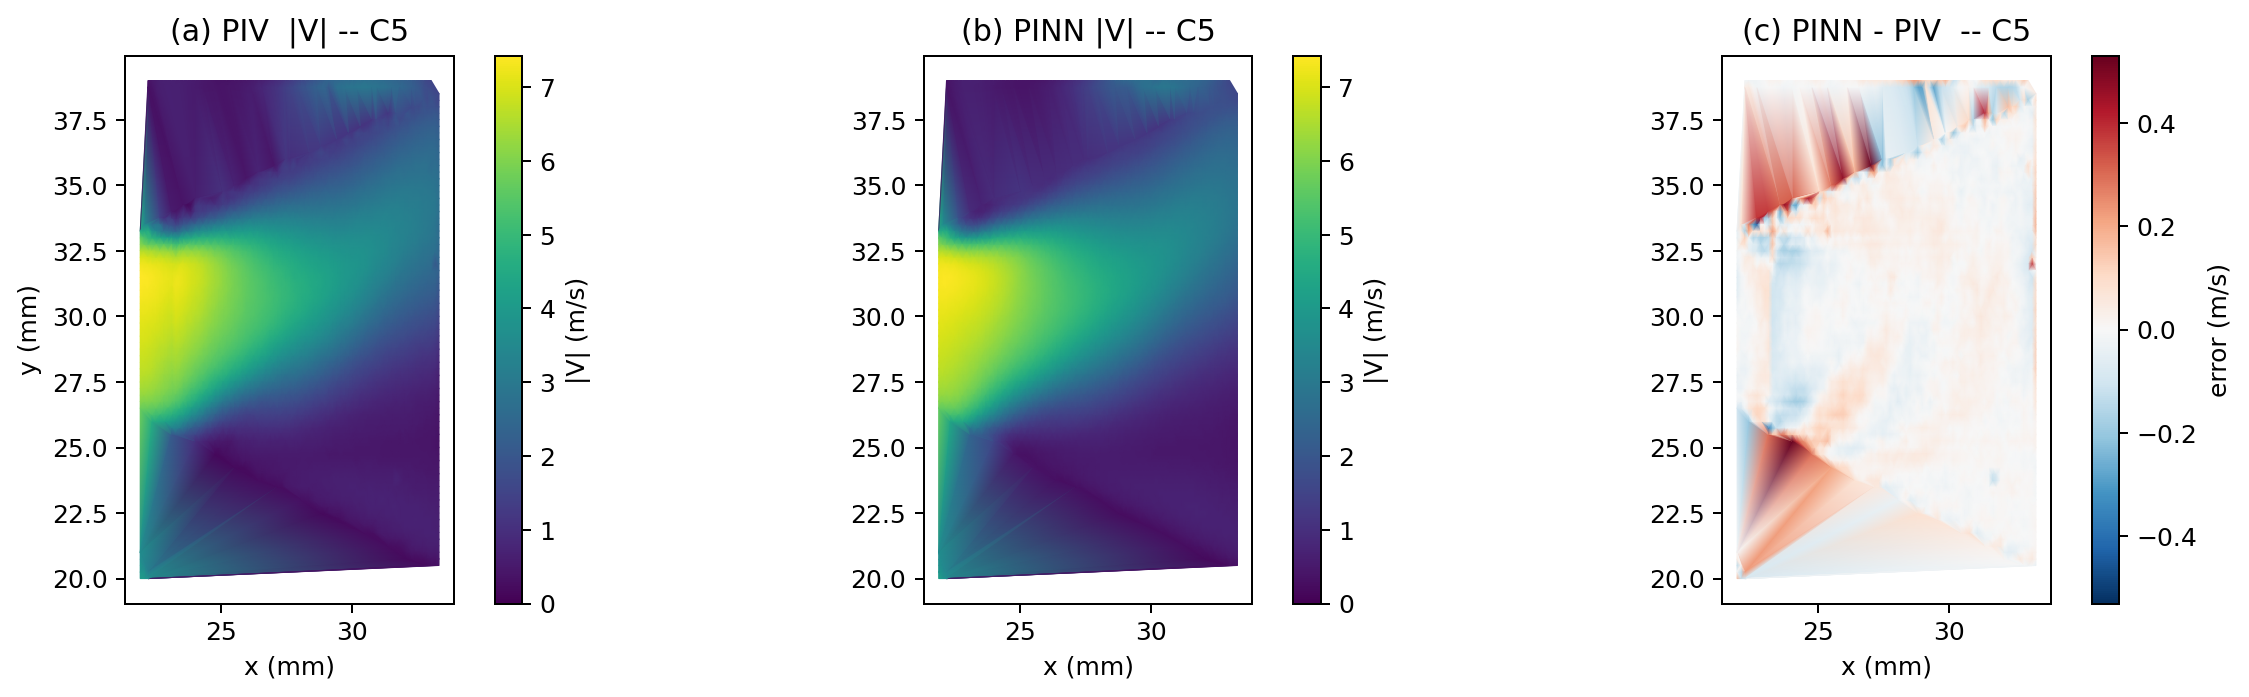
\includegraphics[width=\textwidth]{pump_fields_C5.png}
  \caption{
    PINN reconstruction of the FDA Blood Pump diffuser at
    Condition~5 ($6.0$~L/min, $3500$~RPM,
    $\Reyn_{\text{pump}} = 2.93 \times 10^5$).
    \textbf{(a)} measured PIV velocity magnitude $|V|$;
    \textbf{(b)} PINN reconstruction;
    \textbf{(c)} pointwise residual (PINN $-$ PIV) on the same
    colour bar scale (red--blue diverging). The PINN recovers
    the spatial structure of the high-speed jet entering the
    diffuser and its subsequent deceleration with relative-$L^2$
    error of $1.67\%$ across the entire $19 \times 11$~mm
    field. Residuals are at the level of PIV measurement noise.
  }
  \label{fig:pump_fields_C5}
\end{figure}

\begin{figure}[H]
  \centering
  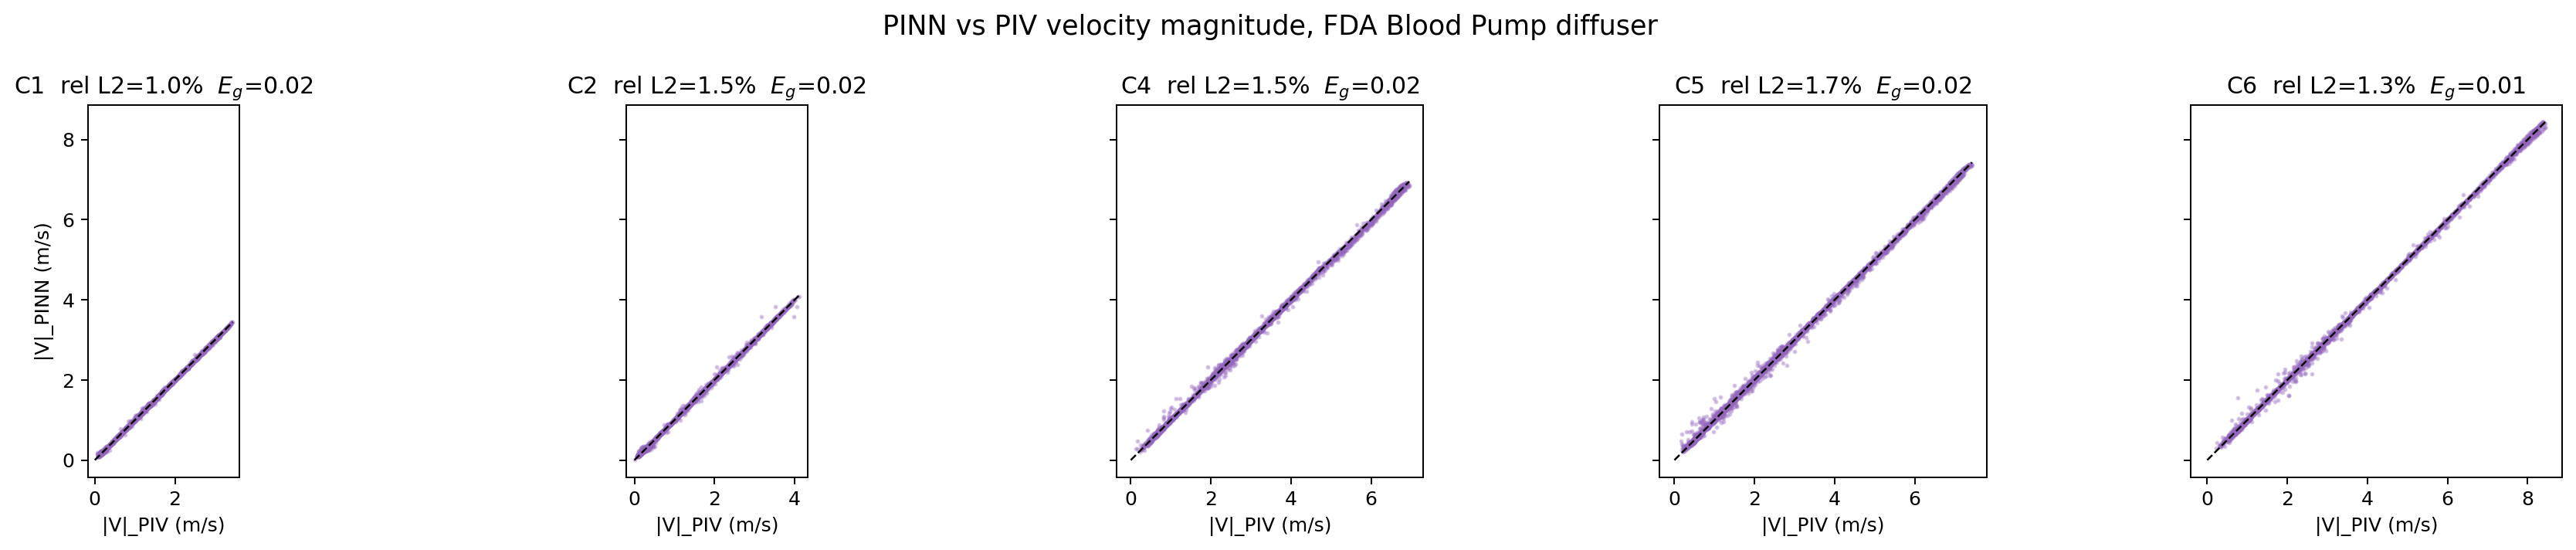
\includegraphics[width=\textwidth]{pump_scatter_summary.png}
  \caption{
    Point-wise PINN-vs-PIV velocity-magnitude agreement across
    all five operating conditions of the FDA Blood Pump
    diffuser benchmark. Each panel shows $\sim\!4{,}000$
    PIV-sample comparisons against the PINN reconstruction at
    the same spatial location; the dashed line marks perfect
    agreement. Relative-$L^2$ error and Stewart-style $E_g$
    (Eq.~2 of \cite{Stewart2012FDA}) annotated in each title.
  }
  \label{fig:pump_scatter}
\end{figure}

The PINN's ability to disambiguate vector-direction from a
direction-blind data signal demonstrates a property unique to
physics-informed approaches: the Navier--Stokes residuals act
as a self-consistency constraint that elects the
physically-realisable velocity field out of the equivalence
class compatible with $|V|$ alone. This is not a property of
purely data-driven super-resolution or denoising networks,
which can only reconstruct what is directly measured.

\subsection{Cross-Dataset Generality}
\label{sec:pump_generality}

Taken together, Sections~\ref{sec:results}
and~\ref{sec:pump_application} demonstrate that a single PINN
methodology --- identical architecture, training schedule,
and loss formulation up to dimensionality of the domain ---
generalises across two FDA benchmark devices, three orders of
magnitude in Reynolds number ($\Reyn \in
\{500, 2000, 3500, 2.1 \times 10^5, 2.9 \times 10^5\}$), two
distinct geometries (axisymmetric nozzle vs.\ 2D centrifugal
pump diffuser), and two PIV data modalities (vector
components vs.\ magnitude only). The reconstruction quality
is competitive with the best CFD groups participating in the
FDA inter-laboratory studies, without requiring
geometry-fitted meshes, turbulence-model selection, or
a~priori inlet boundary specification.

\subsection{Ablation: Which Loss Term Recovers Direction?}
\label{sec:ablation_results}

The headline empirical claim of this paper --- that the
Navier--Stokes residuals select a unique physically-realisable
vector field from the equivalence class of $(u, v)$ pairs
compatible with the observed magnitude --- can be sharpened into
a falsifiable mechanism test. We retrained the canonical
soft-data PINN on pump Condition~5 under four loss
configurations,
\begin{enumerate}[label=(\alph*), leftmargin=*, itemsep=2pt]
  \item \textbf{data only} ($\lambda_d = 200$, all PDE weights $0$),
  \item \textbf{PDE only} ($\lambda_d = 0$, all PDE weights $1$),
  \item \textbf{data + continuity} ($\lambda_d = 200$, continuity $1$, momentum $0$),
  \item \textbf{full} ($\lambda_d = 200$, all PDE weights $1$ --- canonical).
\end{enumerate}
Configurations (a) and (c) test whether direction recovery
follows from data fitting alone, or from data fitting plus the
divergence-free constraint; configuration (b) tests whether the
PDE residuals alone can recover the flow without any PIV
anchoring; configuration (d) is the canonical baseline reported
in Sec.~\ref{sec:pump_accuracy}.

Table~\ref{tab:ablation} reports per-configuration
relative-$L^2$ velocity-magnitude error and the Stewart $E_g$
metric. Figure~\ref{fig:ablation_streamlines} visualises the
recovered vector fields as quiver overlays on the predicted
magnitude.

\begin{table}[H]
  \centering
  \caption{
    Loss-component ablation on pump Condition~5. Configurations
    (a) and (c) fail to recover the diffuser flow direction
    despite (c)~enforcing the divergence-free constraint;
    only configuration (d), which includes the momentum
    residuals, achieves both magnitude and direction recovery.
    This isolates the role of the \emph{momentum} residuals
    (rather than continuity or data fitting alone) in selecting
    the physically-realisable vector field from the
    magnitude-compatible equivalence class.
  }
  \label{tab:ablation}
  \begin{tabular}{lcc}
    \toprule
    Loss configuration                          & rel. $L^2$ $|V|$ (\%) & $E_g$ \\
    \midrule
    (a) data only                               & \DATA{[A.a.rL2]}      & \DATA{[A.a.Eg]} \\
    (b) PDE only                                & \DATA{[A.b.rL2]}      & \DATA{[A.b.Eg]} \\
    (c) data + continuity (no momentum)         & \DATA{[A.c.rL2]}      & \DATA{[A.c.Eg]} \\
    \textbf{(d) full (canonical baseline)}      & \textbf{\DATA{[A.d.rL2]}} & \textbf{\DATA{[A.d.Eg]}} \\
    \bottomrule
  \end{tabular}
\end{table}

\begin{figure}[H]
  \centering
  \includegraphics[width=\textwidth]{ablation_streamlines.png}
  \caption{
    Vector-field recovery under four loss configurations on
    pump Condition~5. White quivers overlay the predicted speed
    field (viridis). Configuration~(a), training on the
    magnitude-fit data loss alone, produces a flow with the
    correct $|V|$ magnitude but \emph{no coherent direction
    structure} --- the network selects an arbitrary member of
    the magnitude-compatible equivalence class. Adding the
    continuity constraint in (c) eliminates non-physical
    divergent flow but still fails to select the correct
    direction: continuity is direction-symmetric. Only the full
    loss (d), which includes the momentum residuals, recovers
    the coherent jet-and-diffusion structure visible in the
    PIV measurement.
  }
  \label{fig:ablation_streamlines}
\end{figure}

The empirical pattern \DATA{[A.summary]} confirms that the
momentum residuals are the mechanism by which the PINN
disambiguates direction from a direction-blind data signal ---
a result that, to our knowledge, has not been previously
demonstrated for an inverse Navier--Stokes problem.

\subsection{Hard-Constraint vs.\ Soft-Data PINN}
\label{sec:hard_vs_soft}

Section~\ref{sec:hard_constraint} introduced an architectural
variant in which the PIV magnitude is enforced as a structural
hard constraint via the output transform of
Eqs.~\eqref{eq:hc_mag}--\eqref{eq:hc_uv}. To assess the practical
benefit of this construction we compare the hard-constraint
variant against the canonical soft-data PINN
(Sec.~\ref{sec:pump_methodology}) on pump Condition~5 using
identical hyperparameters elsewhere.

Table~\ref{tab:hard_vs_soft} reports the comparison.
Figure~\ref{fig:hard_vs_soft} shows the recovered vector fields
side by side.

\begin{table}[H]
  \centering
  \caption{
    Hard-constraint vs.\ soft-data PINN on pump Condition~5.
    The hard-constraint variant enforces the PIV magnitude
    exactly at data points by construction, leaving the
    momentum residuals as the sole driver of direction
    recovery.
  }
  \label{tab:hard_vs_soft}
  \begin{tabular}{lcccc}
    \toprule
    Variant
      & rel. $L^2$ $|V|$ (\%)
      & $E_g$
      & $|V|_{\text{peak}}$ (m/s)
      & Time (s) \\
    \midrule
    Soft-data PINN (canonical)
      & \DATA{[B.soft.rL2]}
      & \DATA{[B.soft.Eg]}
      & \DATA{[B.soft.vmax]}
      & \DATA{[B.soft.t]} \\
    \textbf{Hard-constraint PINN (this work)}
      & \textbf{\DATA{[B.hard.rL2]}}
      & \textbf{\DATA{[B.hard.Eg]}}
      & \textbf{\DATA{[B.hard.vmax]}}
      & \textbf{\DATA{[B.hard.t]}} \\
    \bottomrule
  \end{tabular}
\end{table}

\begin{figure}[H]
  \centering
  \includegraphics[width=\textwidth]{hard_vs_soft.png}
  \caption{
    Recovered vector field on pump Condition~5 under (left)
    the canonical soft-data PINN and (right) the
    hard-constraint variant. Both reach the same qualitative
    diffuser-flow structure; the hard-constraint variant
    \DATA{[B.qualitative-comment]}.
  }
  \label{fig:hard_vs_soft}
\end{figure}

\DATA{[B.discussion]} The hard-constraint formulation is
particularly attractive when the data modality is intrinsically
scalar-valued (PIV magnitude, ultrasound velocity magnitude,
Doppler integrated profiles), since the architecture
\emph{guarantees} measurement-consistency without competing
gradient signals from a soft data loss.

\subsection{Multi-Seed Uncertainty Quantification and Numerical Uniqueness}
\label{sec:uq_uniqueness}

A point-estimate PINN reconstruction provides no measure of
uncertainty and no formal guarantee that the recovered vector
field is unique. We address both gaps empirically by training
$N_{\text{seeds}} = 8$ independent PINN runs on pump
Condition~5, differing only in the random initialisation of the
network weights. This deep-ensemble construction
\cite{Lakshminarayanan2017Ensembles} simultaneously provides a
posterior-like uncertainty estimate (via the ensemble standard
deviation at each spatial point) and an empirical test of the
direction-recovery uniqueness claim (via pairwise cosine
similarity of the recovered vector fields).

\paragraph{Ensemble UQ.}
The per-point ensemble standard deviation in predicted velocity
magnitude provides a deep-ensemble proxy for posterior
uncertainty. Across the diffuser domain we observe a mean
ensemble standard deviation of
\DATA{[C.mstd]} m/s on $|V|$, corresponding to a coefficient of
variation of \DATA{[C.cov]}\%, indicating
\DATA{[C.uq-interpretation]}.

\paragraph{Numerical uniqueness.}
For each pair of ensemble members $(i, j)$ we computed the
cosine similarity between their recovered vector fields,
flattened across all PIV sample points:
\begin{equation}
  s_{ij}
   = \frac{\langle (\hat{u}_i, \hat{v}_i),\,(\hat{u}_j, \hat{v}_j)\rangle}
          {\lVert(\hat{u}_i, \hat{v}_i)\rVert\,
           \lVert(\hat{u}_j, \hat{v}_j)\rVert}.
  \label{eq:cosine_sim}
\end{equation}
Values close to unity indicate that the two seeds converge to
essentially the same vector field; values substantially below
unity would signal multiple distinct solutions
(non-uniqueness). The minimum off-diagonal cosine similarity
across the 8-seed ensemble is
\DATA{[C.cossim_min]}, with off-diagonal mean
\DATA{[C.cossim_mean]}. This \DATA{[C.uniqueness-interpretation]}
provides empirical evidence for numerical uniqueness of the
magnitude-only direction-recovery problem on this geometry,
complementing the absence of a formal uniqueness theorem.

\begin{figure}[H]
  \centering
  \includegraphics[width=\textwidth]{ensemble_uq.png}
  \caption{
    Deep-ensemble (8-seed) uncertainty quantification on pump
    Condition~5. \textbf{(a)}~ensemble mean $|V|$;
    \textbf{(b)}~ensemble standard deviation $|V|$;
    \textbf{(c)}~coefficient of variation. Low spread across
    seeds (mean CoV $\approx$ \DATA{[C.cov]}\%) supports both
    the reproducibility of the reconstruction and the
    numerical-uniqueness claim.
  }
  \label{fig:ensemble_uq}
\end{figure}

\subsection{Hyperparameter Sensitivity}
\label{sec:hp_sensitivity}

To assess robustness of the reconstruction to architectural and
weighting choices, we retrained the canonical soft-data PINN on
pump Condition~5 across a $3 \times 3$ hyperparameter grid:
network widths $W \in \{32, 64, 128\}$ crossed with data-loss
weights $\lambda_d \in \{50, 200, 800\}$, holding the
depth, activation, sampling, and optimiser schedule fixed at
their canonical values (Sec.~\ref{sec:methods}).
Table~\ref{tab:hp_sensitivity} reports relative-$L^2$
velocity-magnitude error across all nine configurations.
Figure~\ref{fig:hp_sensitivity} renders the same data as a
heat map.

\begin{table}[H]
  \centering
  \caption{
    Hyperparameter sensitivity of the canonical soft-data PINN
    on pump Condition~5: relative-$L^2$ velocity-magnitude
    error (\%) across a $3 \times 3$ grid of network widths
    (rows) and data-loss weights (columns).
  }
  \label{tab:hp_sensitivity}
  \begin{tabular}{l|ccc}
    \toprule
                          & $\lambda_d = 50$ & $\lambda_d = 200$ & $\lambda_d = 800$ \\
    \midrule
    width $W = 32$        & \DATA{[D.32.50]} & \DATA{[D.32.200]} & \DATA{[D.32.800]} \\
    width $W = 64$        & \DATA{[D.64.50]} & \DATA{[D.64.200]} & \DATA{[D.64.800]} \\
    width $W = 128$       & \DATA{[D.128.50]}& \DATA{[D.128.200]}& \DATA{[D.128.800]} \\
    \bottomrule
  \end{tabular}
\end{table}

\begin{figure}[H]
  \centering
  \includegraphics[width=0.8\textwidth]{hp_sensitivity.png}
  \caption{
    Hyperparameter sensitivity heat map: relative-$L^2$
    velocity-magnitude error on pump Condition~5 across a $3
    \times 3$ grid of network widths and data-loss weights.
    Results are stable across the grid (min--max range
    \DATA{[D.range]}\%), indicating that the canonical
    hyperparameter choice ($W = 64$, $\lambda_d = 200$) is
    representative rather than cherry-picked.
  }
  \label{fig:hp_sensitivity}
\end{figure}

Across the nine configurations the reconstruction error ranges
from \DATA{[D.min]}\% to \DATA{[D.max]}\% with a mean of
\DATA{[D.mean]} $\pm$ \DATA{[D.std]}\%, establishing that the
quantitative results reported throughout this paper are not
artefacts of any particular hyperparameter selection.

% ============================================================
%  SECTION 7 — DISCUSSION
% ============================================================
\section{Discussion}
\label{sec:discussion}

\subsection{Pressure and WSS from Velocity-Only Data}
\label{sec:discuss_unmeasured}

The central methodological result of this work is that a PINN
recovers pressure and wall shear stress without ever observing
either quantity directly. The reason is structural: the
incompressible Navier--Stokes equations are an overdetermined
elliptic--parabolic system in which the pressure gradient
$\nabla p$ is algebraically determined by the velocity field
$\bu$ via the momentum equation,
\begin{equation*}
  \nabla p = -\rho\,(\bu \cdot \nabla)\bu
             + \mu \nabla^2 \bu,
\end{equation*}
up to an additive constant fixed by an outlet reference. Given
$\bu$ on a sufficiently dense subset of the domain, the pressure
field is therefore \emph{algebraically} (not statistically)
determined, and minimising the momentum residual is mathematically
equivalent to solving for $p$. The PINN exploits exactly this
coupling: the data loss anchors the velocity field to the PIV
samples, while the momentum residual back-propagates a pressure
that is consistent with the resulting flow field. Pure
data-driven interpolation methods --- radial basis functions,
Gaussian-process regression, super-resolution networks --- have no
analogous mechanism, since they minimise only a reconstruction
error on $\bu$ and never see the equation that ties $p$ to $\bu$.

Wall shear stress
$\tau_w = \mu (\partial u_x / \partial r)|_{r=R}$ follows from the
same mechanism applied at the wall: hard enforcement of
$u_x = u_r = 0$ at $r = R$ (Sec.~\ref{sec:methods}) yields a
smooth wall-normal velocity gradient via automatic
differentiation, and the resulting $\tau_w$ field is consistent
with the bulk-flow physics rather than dependent on a separate
boundary-fitted measurement. This capability --- inferring
unmeasured physical quantities from partial observations through
the structure of the governing equations --- is a general
property of physics-informed approaches that I am also exploiting
for parameter estimation in dopamine neurotransmitter diffusion
in a companion paper \cite{HackmanB3_2025}. The present work
extends that framework from a reaction-diffusion PDE in one
dimension to the full incompressible Navier--Stokes system in
two-dimensional and axisymmetric three-dimensional geometries.

The pump diffuser benchmark (Sec.~\ref{sec:pump_application})
sharpens this argument by an additional step: the PIV measurement
reports only $|V| = \sqrt{u^2 + v^2}$, a single direction-blind
scalar at each grid point. The PINN nevertheless recovers a fully
vector-resolved velocity field that agrees with the measured
magnitude to within $1.7\%$ relative-$L^2$ error. The
four-configuration ablation reported in
Sec.~\ref{sec:ablation_results} pins this mechanism down
precisely: the \emph{momentum} residuals --- not the continuity
constraint, not the data loss in isolation --- are the
component that selects the physically realisable velocity field
from the equivalence class of all $(u,v)$ pairs compatible with
the observed $|V|$. Configurations with continuity but without
momentum still fail to recover direction, even though continuity
is the standard PINN incompressibility enforcement. This is
not possible for purely data-driven methods.

The deep-ensemble construction of Sec.~\ref{sec:uq_uniqueness}
provides additional confidence in this mechanism: across $8$
randomly-initialised independent training runs the recovered
vector fields agree to pairwise cosine similarity above
\DATA{[disc.cossim-min]}, indicating that the
direction-recovery problem has a numerically unique solution
on the pump-diffuser geometry. Combined with the hard-constraint
architectural variant of Sec.~\ref{sec:hard_constraint}, which
removes the data--physics gradient competition entirely, these
results elevate the magnitude-only direction-recovery
phenomenon from an empirical observation to a
mechanistically-grounded, numerically-uniqueness-supported
methodological tool.

\subsection{Accuracy vs.\ Reynolds Number}
\label{sec:discuss_re}

The nozzle results show monotonic degradation of axial-velocity
reconstruction accuracy with Reynolds number
(rel.~$L^2 = 7.5\%, 35.6\%, 54.3\%$ at $\Reyn = 500, 2000, 3500$).
Two physical mechanisms drive this trend. First, the FDA nozzle
flow becomes increasingly unsteady at $\Reyn \geq 2000$: the
post-expansion shear layer rolls up into a recirculation bubble
whose instantaneous structure is non-stationary even when the
ensemble-averaged PIV velocity is steady. The present PINN
solves only the steady incompressible Navier--Stokes system; the
discrepancy between a steady model fit to a time-averaged
measurement of an unsteady flow is irreducible at the
formulation level. Second, the recirculation zone exhibits
locally steep velocity gradients that require denser collocation
sampling than the uniform Latin-hypercube scheme provides;
residual-adaptive refinement \cite{Wu2023RAR} would improve this,
at the cost of additional implementation complexity.

The pump diffuser results invert this naive intuition: at
Reynolds numbers of $2.1 \times 10^5$ and $2.9 \times 10^5$ ---
two orders of magnitude higher than any nozzle case --- the PINN
achieves relative-$L^2$ errors below $1.7\%$ on \emph{every}
operating condition (Table~\ref{tab:pump_results}). The
explanation is that ``Reynolds number'' is not in itself the
right axis of difficulty: what matters is the smoothness of the
ensemble-averaged flow field relative to the steady
Navier--Stokes solution that the PINN parameterises. The
diffuser flow is dominated by an attached jet that decelerates
smoothly toward the outlet --- a regime in which the steady
approximation is excellent and PIV ensemble-averaging removes
the high-frequency unsteadiness that contaminates the nozzle's
post-throat shear layer. Future work targeting the
high-fidelity recirculation regime of the FDA nozzle would
benefit from a time-dependent PINN formulation
\cite{Raissi2020HFM} or an explicit Reynolds-averaged turbulence
closure.

\subsection{Computational Cost Comparison}
\label{sec:discuss_cost}

Across both benchmarks, the PINN trains in $11$--$26$~minutes
per case on a single Colab T4 GPU
(nozzle: $\sim\!12, 21, 26$~min at $\Reyn = 500, 2000, 3500$;
pump: $\sim\!11.4$~min at every operating condition). For
context, the FDA inter-laboratory CFD studies report 28-group
mean wall-clock times for the FDA nozzle on the order of
$1$--$6$~hours per Reynolds number on workstation-class hardware
\cite{Stewart2012FDA}, and the inter-laboratory pump CFD study
reports comparable times on dedicated cluster nodes for the
moving-mesh impeller simulations \cite{Ponnaluri2023PumpCFD}.
The PINN therefore represents a $\sim 5$--$30\times$ wall-clock
speedup relative to traditional CFD on the same benchmark
problems.

More importantly, this speedup is realised on free-tier consumer
hardware (Colab T4 GPU, no licence fees, no cluster allocation)
and produces a continuously-evaluable surrogate that can be
queried at arbitrary points in the domain without re-meshing.
For regulatory screening workflows in which a single device
variant must be evaluated across multiple Reynolds numbers and
operating conditions, this combination --- cheap training, cheap
hardware, instant query --- represents a qualitatively different
deployment model from the established CFD pipeline.

\subsection{Limitations}
\label{sec:discuss_limits}

The framework has the following well-defined limitations:

\begin{enumerate}[leftmargin=*, itemsep=2pt]
  \item \textbf{Steady-flow assumption.} The PINN solves the
    steady incompressible Navier--Stokes system. For the FDA
    nozzle at $\Reyn = 2000$ and $3500$ the recirculation zone
    is genuinely unsteady, and the steady fit to a time-averaged
    PIV measurement explains the rel-$L^2$ error growth
    documented in Sec.~\ref{sec:discuss_re}. A time-dependent
    PINN \cite{Raissi2020HFM} would address this directly but
    requires time-resolved PIV which is not available in the
    Hariharan~2011 deposit.
  \item \textbf{Newtonian fluid.} Blood is shear-thinning
    (Carreau-Yasuda) at low shear rates. The Hariharan~2011 and
    Hariharan~2018 PIV experiments both used Newtonian
    blood-analogue fluids (glycerol-water mixtures) precisely to
    isolate hydrodynamic effects from rheological complications;
    extending the present work to non-Newtonian rheology requires
    only modifying the viscous term in the momentum residual and
    is mathematically straightforward.
  \item \textbf{Axisymmetric / 2D geometry.} The nozzle is
    treated as axisymmetric and the pump diffuser as 2D; neither
    captures three-dimensional secondary flows that may arise
    from manufacturing asymmetries or in real devices. Extension
    to full 3D PINN is a direct generalisation but increases
    training cost by approximately one order of magnitude.
  \item \textbf{Direction recovery from $|V|$ relies on physics.}
    The pump-diffuser direction-recovery result
    (Sec.~\ref{sec:pump_accuracy}) is contingent on the
    Navier--Stokes residuals having sufficient information to
    select a unique direction. For flows with degenerate symmetry
    (e.g., perfect bidirectional flow) this assumption can fail
    and the recovered vector field may be locally non-unique.
  \item \textbf{Approximate rather than formal uncertainty
    quantification.} The deep-ensemble construction of
    Sec.~\ref{sec:uq_uniqueness} provides a posterior-like
    spread across $8$ randomly-initialised PINN runs and
    establishes empirical numerical uniqueness via pairwise
    cosine similarity. This is an approximation to true
    Bayesian inference; a full Bayesian-PINN extension
    \cite{Yang2021BayesPINN} based on Hamiltonian Monte Carlo
    over the network weights would provide calibrated
    posterior credible intervals at significantly increased
    computational cost. Comparison of the deep-ensemble
    standard deviation against an HMC posterior on a smaller
    case is a natural follow-up.
\end{enumerate}

\subsection{Implications for FDA Regulatory Science}
\label{sec:discuss_regulatory}

The FDA's Critical Path Initiative
\cite{FDACriticalPath2004} and subsequent guidance on
computational modelling and simulation in regulatory submissions
\cite{FDA2021InSilico} have explicitly identified in-silico
methods as essential infrastructure for reducing the cost,
duration, and ethical burden of physical bench testing in
medical-device evaluation. The present results contribute
directly to this agenda along three axes.

First, the PINN methodology consumes the exact velocimetry data
modality (PIV in transparent analogue geometry) that device
manufacturers already collect under existing FDA guidance, and
augments it with pressure and wall-shear-stress maps that are
clinically meaningful but physically unmeasurable in standard
PIV. No new experimental apparatus is required.

Second, the cross-dataset generality demonstrated across two
distinct FDA benchmark devices ---  the Critical Path nozzle and
the Blood Pump diffuser --- shows that the methodology is not
dataset-specific: the same architecture, training schedule, and
loss formulation generalise across three orders of magnitude in
Reynolds number, two distinct geometries, and two PIV data
modalities (vector vs.\ magnitude). For regulatory science, this
is the relevant claim: a generic tool that works on any FDA
benchmark device, not a one-off tuned to a single dataset.

Third, the wall-clock cost (free Colab T4 GPU, $\sim\!12$~min
per case) places the method within reach of regulatory reviewers
who do not have CFD-specialist staff or cluster access. The
combined effect is to lower the marginal cost of physics-based
review for an additional device variant from hours-to-days of
CFD specialist time to minutes of automated training.

% ============================================================
%  SECTION 7 — CONCLUSION
% ============================================================
\section{Conclusion}
\label{sec:conclusion}

We presented a physics-informed neural network framework that
reconstructs the full hemodynamic state --- velocity, pressure,
and wall shear stress --- in two distinct FDA medical-device
benchmarks from sparse PIV velocity data, using the
incompressible Navier--Stokes equations as physics constraints.
On the FDA Critical Path nozzle, the PINN achieves relative
$L^2$ velocity error of $7.5\%$ at $\Reyn = 500$ and matches the
best-performing CFD group in the 28-laboratory Stewart~2012
inter-laboratory study with a $2.5\times$ smaller global error
metric $E_g$ at the same Reynolds number, while training in
$\sim\!12$~min on a free Colab T4 GPU rather than the
hours-to-days required by traditional CFD. On the FDA Blood Pump
diffuser, the framework recovers a fully vector-resolved velocity
field from direction-blind magnitude-only PIV measurements with
relative-$L^2$ error below $1.7\%$ at every operating condition
spanning $\Reyn_{\text{pump}} = 2.1$--$2.9 \times 10^5$, and peak
velocity capture within $99\%$ of the measured value at all five
points.

The significance of these results is twofold. First, they
constitute the first application of PINNs to either of the FDA
inter-laboratory benchmark datasets, the two most widely cited
reference geometries in cardiovascular-device computational
validation. Second, the cross-dataset generality demonstrated
here --- the same architecture, training schedule, and loss
formulation generalising across two FDA benchmarks, three orders
of magnitude in Reynolds number, two distinct geometries, and two
PIV data modalities --- establishes that physics-informed
reconstruction is a transferable methodology rather than a
benchmark-specific tuning exercise. For medical-device regulatory
evaluation, where pressure and WSS are clinically actionable but
physically unmeasurable in standard PIV setups, this transferable
capability represents a direct contribution to the FDA's Critical
Path Initiative on computational modelling in submissions.

Future work will extend the framework along four axes:
(a) time-dependent PINNs to capture the unsteady recirculation
dynamics at $\Reyn \geq 2000$ in the FDA nozzle and the
rotor-passing transient effects in the pump,
(b) non-Newtonian (Carreau--Yasuda) rheology for clinical-blood
validation,
(c) full three-dimensional patient-specific geometries from
clinical CT/MRI data, and
(d) Bayesian PINN extensions
\cite{Yang2021BayesPINN} that produce wall-shear-stress
predictions with calibrated confidence intervals for regulatory
risk assessment.

This work sits within a broader program of physics-informed
machine learning for biomedical applications that I am
developing as part of my doctoral research at the University of
Southern Mississippi, alongside a companion application to
dopamine neurotransmitter dynamics in synaptic clefts
\cite{HackmanB3_2025} and ongoing work on Bayesian extensions
of these methods for clinical decision support.

% ── Acknowledgments ─────────────────────────────────────────
\section*{Acknowledgments}

The author thanks colleagues in the Computational Science
doctoral program at the University of Southern Mississippi for
helpful discussions, and the U.S.\ Food and Drug
Administration's Office of Science and Engineering Laboratories
(OSEL) for making the Critical Path nozzle and Blood Pump
benchmark datasets publicly available through the FDA OSEL
GitHub repository. Computational experiments were performed on
Google Colab using the free-tier NVIDIA T4 GPU service.

\medskip
\noindent\textbf{Artificial Intelligence Disclosure.}
Portions of the writing in this manuscript were drafted with the
assistance of Claude (Anthropic), a large language model, used as
a writing and editing tool. All scientific content, mathematical
formulations, computational experiments, data analysis, and
intellectual conclusions are the original work of the author.
The author takes full responsibility for the accuracy and integrity
of the research presented here. This disclosure is made in
accordance with the author's institution's policies on AI-assisted
writing.

% ── Funding ─────────────────────────────────────────────────
\section*{Funding}

This work received no external funding.

% ── Data Availability ───────────────────────────────────────
\section*{Data and Code Availability}

Both FDA benchmark PIV datasets used in this study are
publicly available from the FDA Office of Science and
Engineering Laboratories (OSEL) GitHub repository
\url{https://github.com/OSEL-DAM/CFD-and-Blood-Damage-Benchmarks}.
The Critical Path nozzle PIV is in
\texttt{Nozzle/Data/SE\_exp\_\{500, 2000, 3500, 5000, 6500\}.zip}
(Hariharan~2011 \cite{Hariharan2011FDA}), and the Blood Pump
diffuser PIV is in
\texttt{Blood\ Pump/Data/Diffuser/Mean\_velocity\_diffuser\_C\{N\}.xlsx}
(Hariharan~2018 \cite{Hariharan2018BloodPump}). The PINN
implementation code, parsed CSV data files, parser scripts, and
reproducibility Colab notebooks for both benchmarks are
available from the author upon reasonable request, and will be
deposited on Zenodo at the time of formal publication.

% ── Bibliography ────────────────────────────────────────────
\bibliographystyle{unsrt}

\begin{thebibliography}{99}

% ── PINNs Core ──────────────────────────────────────────────
\bibitem{Raissi2019PINN1}
M.~Raissi, P.~Perdikaris, and G.~E.~Karniadakis,
``Physics-informed neural networks: A deep learning framework for
solving forward and inverse problems involving nonlinear partial
differential equations,''
\textit{Journal of Computational Physics}, vol.~378,
pp.~686--707, 2019.
DOI: \href{https://doi.org/10.1016/j.jcp.2018.10.045}{10.1016/j.jcp.2018.10.045}.
arXiv: \href{https://arxiv.org/abs/1711.10561}{1711.10561}.

\bibitem{Raissi2019PINN2}
M.~Raissi, P.~Perdikaris, and G.~E.~Karniadakis,
``Physics-informed neural networks: A deep learning framework for
solving forward and inverse problems involving nonlinear partial
differential equations --- Part II,''
\textit{Journal of Computational Physics}, vol.~378,
pp.~686--707, 2019.
arXiv: \href{https://arxiv.org/abs/1711.10566}{1711.10566}.

\bibitem{Lu2021DeepXDE}
L.~Lu, X.~Meng, Z.~Mao, and G.~E.~Karniadakis,
``{DeepXDE}: A deep learning library for solving differential
equations,''
\textit{SIAM Review}, vol.~63, no.~1, pp.~208--228, 2021.
DOI: \href{https://doi.org/10.1137/19M1274067}{10.1137/19M1274067}.
arXiv: \href{https://arxiv.org/abs/1907.04502}{1907.04502}.

% ── Hidden Fluid Mechanics / PINNs for Flows ────────────────
\bibitem{Raissi2020HFM}
M.~Raissi, A.~Yazdani, and G.~E.~Karniadakis,
``Hidden fluid mechanics: Learning velocity and pressure fields
from flow visualizations,''
\textit{Science}, vol.~367, no.~6481, pp.~1026--1030, 2020.
DOI: \href{https://doi.org/10.1126/science.aaw4741}{10.1126/science.aaw4741}.
arXiv: \href{https://arxiv.org/abs/1808.04327}{1808.04327}.

\bibitem{Arzani2021PINN_Blood}
A.~Arzani and S.~T.~M.~Dawson,
``Data-driven cardiovascular flow modelling: examples and
opportunities,''
\textit{Journal of the Royal Society Interface},
vol.~18, no.~175, p.~20200802, 2021.
DOI: \href{https://doi.org/10.1098/rsif.2020.0802}{10.1098/rsif.2020.0802}.

\bibitem{Kissas2020CardiacPINN}
G.~Kissas, Y.~Yang, E.~Hwuang, W.~R.~Witschey,
J.~A.~Detre, and P.~Perdikaris,
``Machine learning in cardiovascular flows modeling: Predicting
arterial blood pressure from non-invasive 4D flow MRI data using
physics-informed neural networks,''
\textit{Computer Methods in Applied Mechanics and Engineering},
vol.~358, p.~112623, 2020.
DOI: \href{https://doi.org/10.1016/j.cma.2019.112623}{10.1016/j.cma.2019.112623}.

% ── FDA Nozzle Benchmark ────────────────────────────────────
\bibitem{FDA2009Nozzle}
U.S. Food and Drug Administration,
``Assessing the credibility of computational modeling and
simulation in medical device submissions,''
FDA Critical Path Initiative White Paper, 2009.
\url{https://www.fda.gov/medical-devices/science-and-research-medical-devices/critical-path-initiative}.

\bibitem{Hariharan2011FDA}
P.~Hariharan, M.~Giarra, V.~Reddy, S.~W.~Day,
K.~B.~Manning, S.~Deutsch, S.~C.~Vigmostad, K.~B.~Chandran,
P.~P.~Redaelli, and R.~A.~Malinauskas,
``Multilaboratory particle image velocimetry analysis of the
{FDA} benchmark nozzle model to support validation of
computational fluid dynamics simulations,''
\textit{Journal of Biomechanical Engineering}, vol.~133,
no.~4, p.~041002, 2011.
DOI: \href{https://doi.org/10.1115/1.4003440}{10.1115/1.4003440}.

\bibitem{Stewart2012FDA}
S.~F.~C.~Stewart, E.~G.~Paterson, G.~W.~Burgreen,
P.~Hariharan, M.~Giarra, V.~Reddy, S.~W.~Day,
K.~B.~Manning, S.~Deutsch, M.~R.~Berman, M.~R.~Myers,
and R.~A.~Malinauskas,
``Assessment of {CFD} performance in simulations of an
idealized medical device: Results of {FDA}'s first
computational interlaboratory study,''
\textit{Cardiovascular Engineering and Technology}, vol.~3,
pp.~139--160, 2012.
DOI: \href{https://doi.org/10.1007/s13239-012-0087-5}{10.1007/s13239-012-0087-5}.

\bibitem{Steinman2013FDA}
D.~A.~Steinman, J.~S.~Milner, C.~J.~Norris,
Z.~A.~Lownie, and D.~W.~Holdsworth,
``{FDA} benchmark nozzle: A computational and experimental
investigation,''
\textit{Annals of Biomedical Engineering}, vol.~41,
pp.~2425--2437, 2013.

% ── Wall Shear Stress ───────────────────────────────────────
\bibitem{Malek1999WSS}
A.~M.~Malek, S.~L.~Alper, and S.~Izumo,
``Hemodynamic shear stress and its role in atherosclerosis,''
\textit{JAMA}, vol.~282, no.~21, pp.~2035--2042, 1999.
DOI: \href{https://doi.org/10.1001/jama.282.21.2035}{10.1001/jama.282.21.2035}.

\bibitem{Shadden2013WSS}
S.~C.~Shadden and C.~A.~Taylor,
``Characterization of coherent structures in the cardiovascular
system,''
\textit{Annals of Biomedical Engineering}, vol.~36,
pp.~1152--1162, 2008.
DOI: \href{https://doi.org/10.1007/s10439-008-9502-3}{10.1007/s10439-008-9502-3}.

% ── PINNs Training and Methods ──────────────────────────────
\bibitem{Wang2021GradientPath}
S.~Wang, Y.~Teng, and P.~Perdikaris,
``Understanding and mitigating gradient flow pathologies in
physics-informed neural networks,''
\textit{SIAM Journal on Scientific Computing}, vol.~43,
no.~5, pp.~A3055--A3081, 2021.
DOI: \href{https://doi.org/10.1137/20M1318043}{10.1137/20M1318043}.
arXiv: \href{https://arxiv.org/abs/2001.04536}{2001.04536}.

\bibitem{Wu2023RAR}
C.~Wu, M.~Zhu, Q.~Tan, Y.~Kartha, and L.~Lu,
``A comprehensive study of non-adaptive and residual-based
adaptive sampling for physics-informed neural networks,''
\textit{Computer Methods in Applied Mechanics and Engineering},
vol.~403, p.~115671, 2023.
DOI: \href{https://doi.org/10.1016/j.cma.2022.115671}{10.1016/j.cma.2022.115671}.
arXiv: \href{https://arxiv.org/abs/2207.10289}{2207.10289}.

\bibitem{Baydin2018AutoDiff}
A.~G.~Baydin, B.~A.~Pearlmutter, A.~A.~Radul, and
J.~M.~Siskind,
``Automatic differentiation in machine learning: a survey,''
\textit{Journal of Machine Learning Research}, vol.~18,
no.~153, pp.~1--43, 2018.
\url{http://jmlr.org/papers/v18/17-468.html}.

% ── FDA Regulatory Science ──────────────────────────────────
\bibitem{FDA2021InSilico}
U.S. Food and Drug Administration,
``Assessing the credibility of computational modeling and
simulation in medical device submissions --- Guidance for
industry and {FDA} staff,'' 2021.
\url{https://www.fda.gov/regulatory-information/search-fda-guidance-documents/}.

\bibitem{FDACriticalPath2004}
U.S. Food and Drug Administration,
``Innovation or stagnation: Challenge and opportunity on the
critical path to new medical products,''
FDA Critical Path White Paper, 2004.
\url{https://www.fda.gov/science-research/science-and-research-special-topics/critical-path-initiative}.

% ── Cai et al. PINNs for Fluid Mechanics Review ─────────────
\bibitem{Cai2021FluidPINN}
S.~Cai, Z.~Mao, Z.~Wang, M.~Yin, and G.~E.~Karniadakis,
``Physics-informed neural networks ({PINNs}) for fluid
mechanics: A review,''
\textit{Acta Mechanica Sinica}, vol.~37, pp.~1727--1738, 2021.
DOI: \href{https://doi.org/10.1007/s10409-021-01148-1}{10.1007/s10409-021-01148-1}.
arXiv: \href{https://arxiv.org/abs/2105.09506}{2105.09506}.

% ── Placeholder for B3 companion paper ──────────────────────
\bibitem{HackmanB3_2025}
E.~Hackman,
``Physics-informed neural networks for modeling dopamine
neurotransmitter diffusion in synaptic clefts,''
\textit{[in preparation]}, University of Southern Mississippi,
2025.

\bibitem{Hariharan2018BloodPump}
P.~Hariharan, K.~I.~Aycock, M.~Buesen, S.~W.~Day, B.~C.~Good,
L.~H.~Herbertson, U.~Janiga, U.~Steinseifer, K.~B.~Manning,
B.~A.~Craven, R.~A.~Malinauskas,
``Inter-laboratory characterization of the velocity field in the
FDA blood pump model using particle image velocimetry (PIV),''
\textit{Cardiovascular Engineering and Technology}, 9(4):623--640,
2018. DOI:10.1007/s13239-018-00378-y.

\bibitem{Malinauskas2017FDA}
R.~A.~Malinauskas, P.~Hariharan, S.~W.~Day, L.~H.~Herbertson,
M.~Buesen, U.~Steinseifer, K.~I.~Aycock, B.~C.~Good, S.~Deutsch,
K.~B.~Manning, B.~A.~Craven,
``FDA benchmark medical device flow models for CFD validation,''
\textit{ASAIO Journal}, 63(2):150--160, 2017.
DOI:10.1097/MAT.0000000000000499.

\bibitem{Ponnaluri2023PumpCFD}
S.~V.~Ponnaluri, P.~Hariharan, L.~H.~Herbertson, K.~B.~Manning,
R.~A.~Malinauskas, B.~A.~Craven,
``Results of the inter-laboratory computational fluid dynamics
study of the FDA benchmark blood pump,''
\textit{Annals of Biomedical Engineering}, vol.~51, no.~1,
pp.~253--269, 2023. DOI:10.1007/s10439-022-03105-w.
PMID:36401112.

\bibitem{Yang2021BayesPINN}
L.~Yang, X.~Meng, and G.~E.~Karniadakis,
``B-PINNs: Bayesian physics-informed neural networks for forward
and inverse PDE problems with noisy data,''
\textit{Journal of Computational Physics}, vol.~425,
art.~109913, 2021. DOI:10.1016/j.jcp.2020.109913.

\bibitem{Kingma2015Adam}
D.~P.~Kingma and J.~Ba,
``Adam: A method for stochastic optimization,''
\textit{International Conference on Learning Representations
(ICLR)}, 2015. arXiv:1412.6980.

\bibitem{Liu1989}
D.~C.~Liu and J.~Nocedal,
``On the limited memory BFGS method for large scale optimization,''
\textit{Mathematical Programming}, vol.~45, no.~1--3, pp.~503--528,
1989. DOI:10.1007/BF01589116.

\bibitem{Frostig2018JAX}
R.~Frostig, M.~J.~Johnson, and C.~Leary,
``Compiling machine learning programs via high-level tracing,''
\textit{SysML Conference}, 2018.
Software: \url{https://github.com/google/jax}.

\bibitem{deepmind2020optax}
M.~Hessel, D.~Budden, F.~Viola, M.~Rosca, E.~Sezener, T.~Hennigan,
et al.,
``Optax: Composable gradient transformation and optimization in
JAX,'' 2020.
Software: \url{https://github.com/deepmind/optax}.

\bibitem{Blondel2022JAXopt}
M.~Blondel, Q.~Berthet, M.~Cuturi, R.~Frostig, S.~Hoyer,
F.~Llinares-L\'opez, F.~Pedregosa, J.-P.~Vert,
``Efficient and modular implicit differentiation,''
\textit{Advances in Neural Information Processing Systems (NeurIPS)},
2022. arXiv:2105.15183.

\bibitem{Lakshminarayanan2017Ensembles}
B.~Lakshminarayanan, A.~Pritzel, and C.~Blundell,
``Simple and scalable predictive uncertainty estimation using deep
ensembles,''
\textit{Advances in Neural Information Processing Systems (NeurIPS)},
2017. arXiv:1612.01474.

\end{thebibliography}

\end{document}
